\RequirePackage{fix-cm}
%
%\documentclass{svjour3}                     % onecolumn (standard format)
%\documentclass[smallcondensed]{svjour3}     % onecolumn (ditto)
%\documentclass[smallextended]{svjour3}       % onecolumn (second format)
\documentclass[twocolumn]{svjour3}          % twocolumn
\smartqed  % flush right qed marks, e.g. at end of proof
\usepackage{graphicx}
\usepackage[vlined, ruled, boxed]{algorithm2e}
\usepackage{tabularx}
\usepackage{epstopdf}
\journalname{CGI2013} % The correct name will be entered by the editor
\begin{document}

\title{Real-time Virtual Fitting Room Framework With Physics Simulation} 
\subtitle{Application of Real-Time Motion Smoothing and User Measurement}
\author{First Author \and Second Author}
\institute{First Author \at F. Author Address \and Second Author \at S. Author Address}

%\author{Umut G\"{u}ltepe  \and U\u{g}ur G\"{u}d\"{u}kbay}
%\institute{Bilkent University \at Ankara \and Bilkent University \at Ankara}
\date{ }% The correct dates will be entered by the editor

\maketitle

\begin{abstract}
We present our novel virtual fitting room framework using a depth sensor, which provides a realistic fitting experience with customized motion filters, size adjustments and physical simulation. The proposed scaling method adjusts the avatar and determines a specific apparel size, prepares the physics simulation and collision detection environment, with a total preprocessing time of one second, eliminating the requirement for long preprocessing times to achieve a realistic fitting experience. The real-time motion filters prevents unnatural artifacts due to the noise from depth sensor or self-occluded body parts.
\keywords{virtual fitting room \and depth sensor \and character animation  \and motion capture  \and appearance capture}
\end{abstract}

\section{Introduction}
\label{sec:Introduction}
One of the most time-consuming stages of apparel shopping is trying the apparels on, which is not even possible in online stores. With the advances in augmented reality technologies, virtual fitting rooms are slowly taking their places in both real and virtual stores~\cite{Fitnect2012,Styku2013} to improve the quality of apparel trial experience while also making it faster.

Advanced virtual fitting rooms show the apparel items either on the video of the user or on a virtual avatar, both scaled to reflect the user's body characteristics~\cite{FaceCake2013}. Some of them also employ physics-based garment simulation for a better fitting experience~\cite{Styku2013}.

We present a novel virtual fitting room framework which provides all the basic features expected from such an application, along with enhancements in various aspects for higher realism. These enhancements include motion filtering, customized user scaling and physics engine.

The rest of the paper is organized as follows. Section~\ref{sec:Related} presents related work on virtual fitting rooms and depth sensors.
Section~\ref{sec:Overall} provides the outline of the framework and explains the components. 
Section~\ref{sec:Physics} explains the cloth simulation engine and purposes of the user measurements. 
Section~\ref{sec:Measurements} describes the proposed methodology, including the details of depth map filtering, body measurements, and temporal averaging.  
Section~\ref{sec:Motion} illustrates the techniques used for coping with the inferior motion data problems.
Section~\ref{sec:Experiments} provides experimental results. Section~\ref{sec:Conclusions} gives conclusions and further research directions. 

\section{Previous Work}
\label{sec:Related}
Virtual fitting rooms have been a research subject for more than a decade. Protopsaltou~\cite{Protopsaltou2002} developed an Internet-based approach for virtual fitting rooms, although it was not real time and required marker-based motion capture systems for animation. Zhang~\cite{Zhang2008} used a multi-camera system utilizing shell fitting space (SFS)~\cite{Cheung2005} techniques to build a real time intelligent fitting room. 

Advances in time-of-flight technology made depth sensors available at consumer-level prices with better performance. This prompted a wave of research based on depth sensors in various fields, such as rehabilitation~\cite{Yao2011}, indoor modeling~\cite{Henry2012}, and medicine~\cite{Gallo2012}. Another topic that attracted significant attention from both researchers and companies is real-time virtual fitting rooms~\cite{Meng2010}. Giovanni~\cite{Giovanni2012} developed a virtual try-on system utilizing a calibrated set of Kinect and high definition cameras, while comparing the two state-of-the-art depth sensing software development kits (SDKs)-OpenNI~\cite{OpenNI2013} and Kinect for Windows~SDK~\cite{Microsoft2013}. While most frameworks utilize garment meshes with physics simulation \cite{Styku2013,Fitnect2012}, another intriguing approach is using a pre-recorded apparel image database, from which the images are superpositioned onto the RGB video of the user\cite{Zhou2012,Hauswiesner2013}. 

One problem with depth sensors is the feeble quality and noisiness of the depth stream. This problem is analyzed in depth by Khoshelham~\cite{Khoshelham2012} and concluded that the standard deviation reaches two centimeters in a measuring distance of three meters. Matyunin~\cite{Matyunin2011} attempted to improve the quality by filtering with additional information from the attached RGB camera.  

A key purpose of both virtual and real fitting rooms is giving the customer the look and feel of a cloth with a specific size on the the user's body, so the user can choose the appropriate size for him. Embedding the feature of matching cloth sizes with users requires capturing the users' body dimensions. More advanced frameworks even construct virtual avatars with input from only one depth sensor \cite{Cui2013,Cui2010}. On the other hand, despite these works provide higher detail avatars and keener measurements, which might be more suitable for made-to-measure type of framework, the process requires too much time to work with a real-time 'fixed-size try-on' virtual fitting room application where simple body height and width measurements are sufficient. These applications require a faster approach along with a specialized garment design framework such as the work of Yasseen et al.\cite{Yasseen2013} or Meng et al. \cite{Meng2010}. A recent study \cite{Kim2013} shows that such appliations are well-recieved by public and have potential commercial uses.     

\section{Overall Framework}
\label{sec:Overall}
The main objective of a virtual dressing room is giving the user the idea of how the apparel will look on him/her without actually trying it on. As in any simulation, the absolute reality is almost impossible to attain, although with garment simulation and depth sensing technologies, a substantial level of realism can be achieved.

\begin{figure*}
	\centerline{
	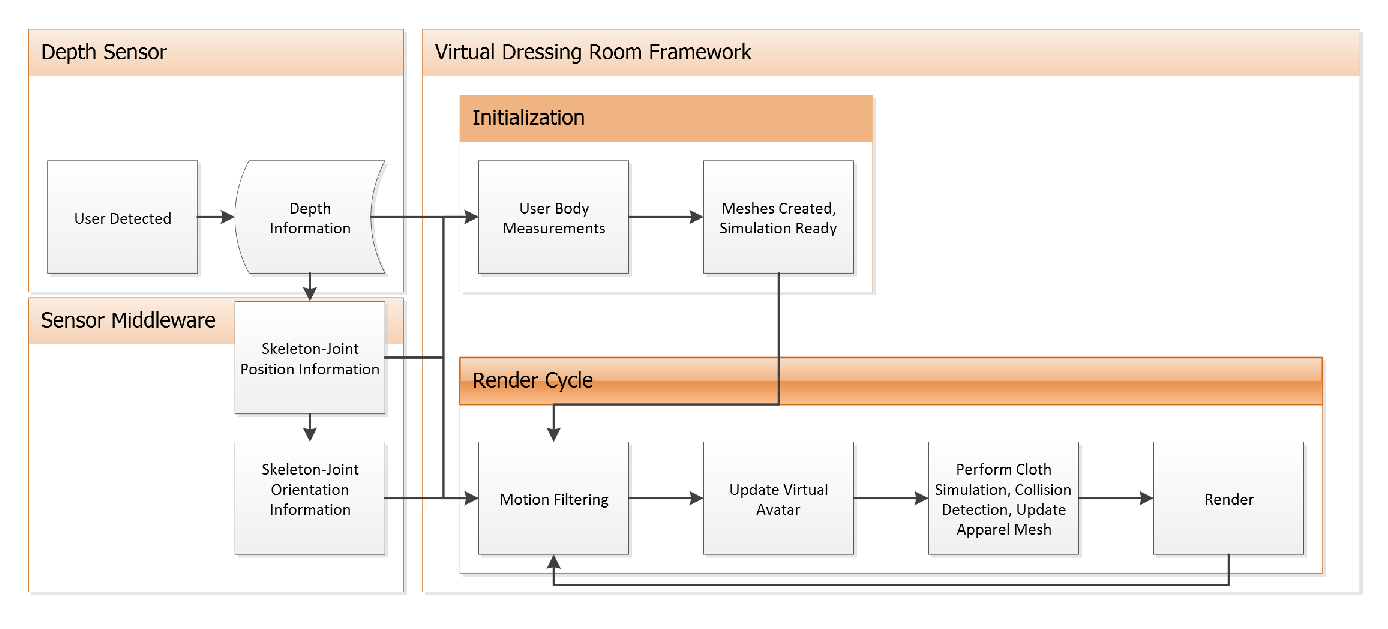
\includegraphics[width=2.0\columnwidth]{./figures/overall.eps}
	}
	\caption{The overall virtual dressing framework}
	\label{fig:overall}
\end{figure*}

The flow diagram of our framework is given in Figure \ref{fig:overall}. The core functions of the framework are:

\begin{itemize}
  \item 3D scene rendering and render cycle management, 
  \item Weighted Skinning and Skeletal Animation,
  \item Depth sensor integration.
\end{itemize}

As these topics are considered boiler plate for such an application, they are not explained in detail in this paper. On the other hand, section \ref{sec:Physics} will give basic information about the embedded physics engine and explain its place within the overall program.  The sections \ref{sec:Motion} and \ref{sec:Measurements} will provide in-depth information and analysis of some of the features developed specifically for this particular application. 


\section{Physics Engine}
\label{sec:Physics}
The cloth simulation framework utilizes the propriety PhysX engine by Nvidia\cite{Kim2011}, with two major components as the cloth deformation and the collision detection. 

The deformation algorithm is based on the Position Based Dynamics by \cite{M�llera2007}, calculating the position of the particles from their previous positions and applying constraints on mutual distance and angle. The approach is stable and efficient for real time applications. 

Collision between the body and the cloth is detected using collision spheres and capsules (composed of two spheres) co-located with body joints and bones, respectively (cf.~Figure \ref{fig:colliders}). The female body bone information is extracted from the input skeletal mesh class, and the colliding capsules are generated automatically after the measurement process, with the capsule pair indexes stored in a read only array.

\begin{figure}
	\begin{center}
	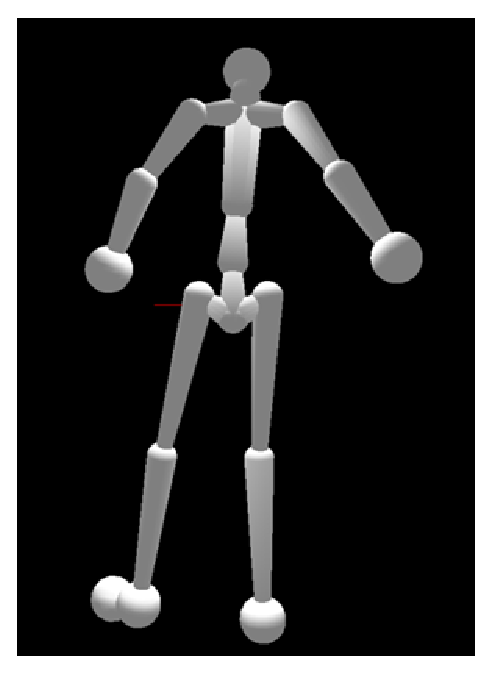
\includegraphics[width=1.0\columnwidth]{./figures/colliders.eps}
	\end{center}
	\caption{The colliding human body with default radii}
	\label{fig:colliders}
\end{figure}

The solution is performed for the trajectory of the capsule or sphere and the particle for frame interval. This approach is especially robust in fast motion, which is important since the motion is created in real time. The required solution is a 6th degree polynomial, which is approximated with quadratic equation. The solution is performed on the GPU, which increases the parallel performance greatly, allowing for higher frame rates than 600 frames per second (fps). The cloth is discretized as a triangle mesh and the collision is only detected on vertices, therefore density must be high enough in order to avoid penetration at locations further from the vertices~\cite{Kim2011,Tonge2010}. This issue can be resolved using the virtual particles for apparel meshes with lower resolution, where additional vertices are introduced at runtime for collision simulation~\cite{Kim2011}.

The acquired body measurements are used to estimate the locations of joints and bones, for collision sphere placement, whereas the radii are used directly for determining the sphere sizes. With both parameters scaled according to the user, various body types can be simulated realistically.

\section{Body Measurements}
\label{sec:Measurements}
For a realistic fitting experience, another requirement is acquiring a set of simulation parameters from a human test-subject for a pre-modeled apparel mesh, which is to be displayed on a virtual avatar reflecting the body characteristics of the aforementioned subject.  The set of parameters for the simulation includes the body height and width, also the radii for the collision spheres, which have their centers coinciding with the joints of the virtual avatar's skeleton.
The body width and height are then utilized to estimate the body size of the user, collision spheres are used in the dressing room simulation, to detect and resolve collision with the cloth particles.

As opposed to works focusing on acquiring high-detail avatars of subjects for made-to measure applications, we focus on the speed of the overall algorithm for real-time purposes and acquire enough measurements for a 'fixed-size try-on' system.   
  
\subsection{Depth Map Filtering}
\label{subsec:4.1} 
The state-of the art time-of-flight (TOF) cameras still provide low resolution and quality output compared to current advanced RGB systems. The quality of the input depth map is a crucial factor on the overall performance of the system, therefore, we first wish to improve the quality of the depth map by applying canonical image optimization methods.

In this approach, we utilize a TOF camera running with a middleware that provides a subject map. The subject map has the same size as the depth map. It has the same origin as the pixels of the depth map, either belonging to a subject or to the background.

Let us take the input depth map $D$ as a $M \times N$ matrix. Initially, the user pixels from $D$ are extracted by a pixel-by-pixel comparison with the input user map. We are only interested in the one subject and $D_1$ represents the depth pixels of him, whereas $U_1$ is the bit map of the subject. Also, the non-subject pixels are set to the mean value of the user pixels, to set the matrix properly for the subsequent filterings.

\begin{equation}
D_1=(D-(D \times U_1 )) \times \frac{1}{n} \times \sum\limits_{i=0}^n \left(\left(D \times U_1 \right)_i + d \times U_1 \right)
\label{eqn:patch_depth}
\end{equation}

The subject depth map is now prepared to be processed with Gaussian filtering to normalize and improve the quality. 

\begin{equation}
D_G\;=\;D_1\;*\;G, 
\label{eqn:gaussian_convolution}
\end{equation}

\noindent where `$*$' is the convolution operator. The Gaussian filtering completes the optimization of the input depth map. 
The overall process is described in Algorithm \ref{algo:depth_patch}.

\begin{algorithm}
\DontPrintSemicolon 
\KwIn{Raw depth and subject stream from the depth sensor}
\KwOut{Optimized subject map}
$depth_{\textit{sum}}=0$ \;
$n_{\textit{user}} =0$\;
\For{i \bf{from} 0 \bf{to} $d_{\textit{width}}$ }{
\For{j \bf{from} 0 \bf{to} $d_{\textit{height}}$ }{
\If{$U(i,j)$} {
  $depth_{\textit{sum}}=depth_{\textit{sum}}+D(i,j)$\;
  $n_{\textit{user}}+=1$\;
 }}}
$depth_{\textit{average}}=depth_{\textit{sum}}/n_{\textit{user}}$ \;
\For{i \bf{from} 0 \bf{to} $d_{\textit{width}}$ }{
\For{j \bf{from} 0 \bf{to} $d_{\textit{height}}$ }{
\If{\bf{not}  $U(i,j)$} {
  $D(i,j)=depth_{\textit{average}}$\;
 }}}
 
\For{i \bf{from} 0 \bf{to} $d_{\textit{width}}$ }{
\For{j \bf{from} 0 \bf{to} $d_{\textit{height}}$ }{
\If{$U(i,j)$} {
  $D(i,j)=D(i-m:i+m, j-n:j+m) * \newline \hspace*{1.35cm} Gaussian(m,n,e)$\;
 }}}
\Return{D}
\caption{Depth Map Filtering}
\label{algo:depth_patch}
\end{algorithm}

\subsection{Body Measurement}
\label{subsec:4.2} 

By now, we have an optimized depth map, which is ready for performing key body dimension measurements. The key dimensions are handled in two groups: the collision sphere radii, which are used for the collision detection in the simulation, and the height and width parameters, which are used to determine to size of the apparel. 

\subsubsection{Collision Sphere Radii}

The simulation framework utilizes collision spheres and capsules instead of arbitrary geometries. This constraint allows the simulation to run in real time with exceptionally high frame rates by simplifying the algorithms. There are a total of 15 joint locations provided by the middleware, as shown in Figure~\ref{fig:nite_joints}. These are the key points for collision sphere placement. For this reason, the framework also utilizes 15 collision spheres and the capsules formed by pairs.

\begin{figure}
	\begin{center}
	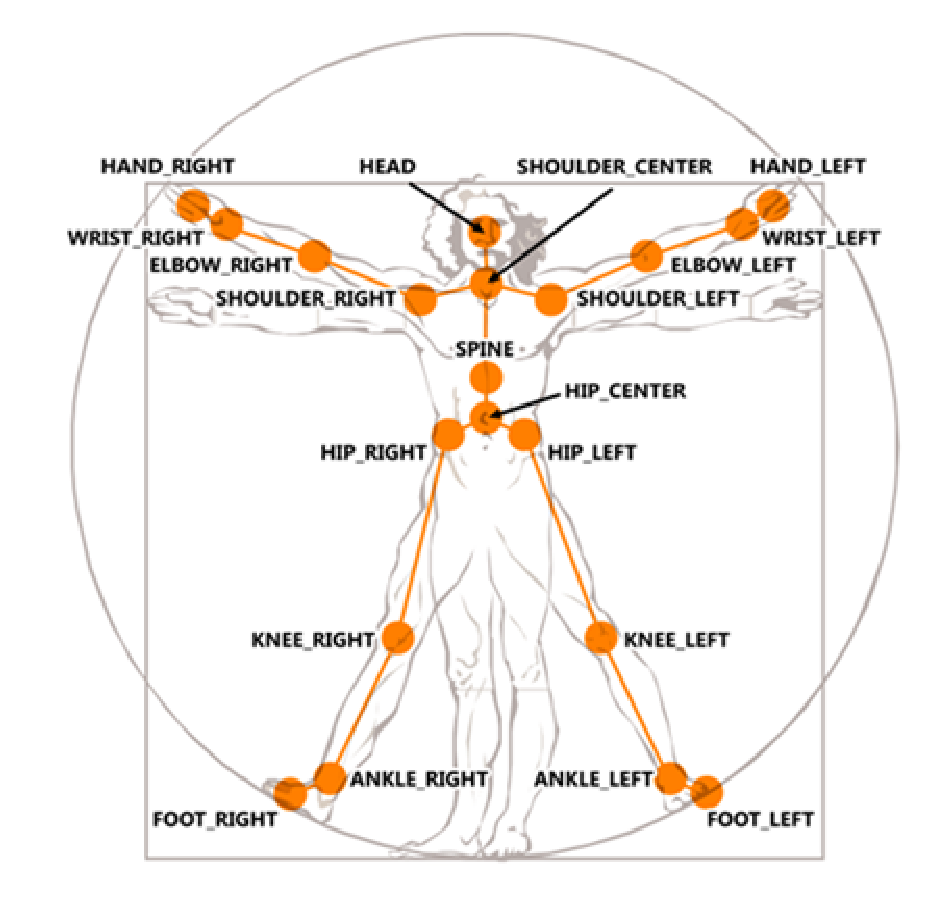
\includegraphics[width=1.0\columnwidth]{./figures/nite_joints.eps}
	\end{center}
	\caption{Human joints provided by NITE~\cite{PS2102}.}
	\label{fig:nite_joints}
\end{figure}


For a realistic simulation, collision spheres must be as large as possible without intersecting the skin mesh of the avatar. The optimal sphere fitting algorithm starts with an infinitely small circle and expands it discretely until it intersects with the body contour. The steps of this algorithm are as follows:  

\begin{enumerate}
\item Take vector $J_i$, which represents the coordinates of the $i^{th}$ joint.
Initialize the radius of the sphere by setting it to the z-distance with the overlapping point in the depth map.
\begin{equation}
r_i^z=J_i^z-D^z(J_i^x,J_i^y)
\label{eqn:z_sphere_radius}
\end{equation}
\item Start with an infinitely small line segment parallel to the x-axis. Expand it until it intersects with the body contour. Take the x-distance between the intersection point and the joint location. Repeat the same process with a line segment parallel to the y-axis and take the larger radius. While expanding the segment, stop expanding and discard the corresponding result if the border of the depth map is reached.
\begin{equation}
r_i^{x,y}=max(|J_i^{x,y} \; - \; D^{x,y}(J_i^{y,x},J_i^z)|)
\label{eqn:x_y_sphere_radius}
\end{equation}
\item Take the minimum of the radii of the three axes because there should be no intersection with the body contour and the shape must be a sphere.
\begin{equation}
r_i=min(r_i^{x, y, z})
\label{eqn:minimum_sphere-radius}
\end{equation}
\end{enumerate}

\noindent The pseudocode of the optimal sphere fitting is given in Algorithm~\ref{algo:sphere_fitting}.

\begin{algorithm}
\DontPrintSemicolon 
\KwIn{Optimized depth stream from the depth sensor}
\KwOut{Collision sphere radii for each joint}
\ForEach{joint}{
$p=pos_{J_m}$\;
$r_z=\sqrt{P_z^2-D_z(P_x,P_y)^2}$\;
\For{i \bf{from} $P_x$ \bf{to} $0$ }{
\If{$D(i,P_y)$ \bf{equals}  $P_z$} {
  $r_{x^{-}} = i$\;
  break\;
 }
}
\For{i \bf{from} $P_x$ \bf{to} $\textit{depth}_{\textit{width}}$ }{
\If{$D(i,P_y)$ \bf{equals}  $P_z$} {
  $r_{x^{+}} = i$\;
  break\;
 }
}
\For{j \bf{from} $P_y$ \bf{to} $0$ }{
\If{$D(P_x,j)$ \bf{equals}  $P_z$} {
  $r_{y^{-}} = j$\;
  break\;
 }
}
\For{j \bf{from} $P_y$ \bf{to} $\textit{depth}_{\textit{height}}$ }{
\If{$D(P_x,j)$ \bf{equals}  $P_z$} {
  $r_{y^{+}} = j$\;
  break\;
 }
}
$r_m=min(r_z,\; r_{x^{-}}, \; r_{x^{+}},\; r_{y^{-}}, \; r_{y^{+}})$
}
\Return $(r_{0}, \; r_{1} \; \ldots \; r_{n})$ 
\caption{Sphere Fitting Algorithm}
\label{algo:sphere_fitting}
\end{algorithm}  

\subsubsection{Height and Width Parameters}

The width and height of the subject is important for determining the proper actual size for the cloth. However, a straightforward 
estimation of the body height and shoulder width is prone to errors due to the noise and quality of the incoming depth map. In 
order to minimize the error factor, an upscaled version of the subject's body is measured, to be used in width-height estimation 
later. We use the human body proportions defined by~\cite{Willis2012}, which are shown in Table~\ref{tbl:human_body_proportions}. 
For the sake of relative representation, the width and height of the head are taken as unit width and height, respectively. The 
measurement source column in the table represents the source for the estimation of the respective parameter:
\begin{itemize} 
\item
The joint location represents that the measurement will take the input subject joint locations as the reference.
\item 
The depth map represents the measurement will instead perform measurements based on the pixel distribution in the filtered subject depth map. 
\end{itemize}
They are often used together for better performance. Please note that some of these parameters are not standard to be used as relative references, such as the hip width. These parameters do not effect others in the estimation process and vice versa.

\begin{table}
\begin{center}
\begin{tabular}{|l|c|c|l|}
\hline
\textbf{Distance} & \textbf{Width} & \textbf{Height} & \textbf{Measurement} \\ 
\textbf{        } & \textbf{     } & \textbf{      } & \textbf{Source} \\ \hline
Head & 1w (1) & 1h (2) & Depth Map + \\ 
     &        &        & Joint Location \\ \hline
Body Height & - & 7h (3) & Depth Map \\ \hline
Hip Height & - & 4h (4) & Joint Location \\ \hline
Elbow to & - & 2h (5) & Depth Map + \\ 
Fingertip &   &       & Joint Location \\ \hline
Wrist to  & - & 1h (6) & Depth Map + \\ 
Fingertip &   &       & Joint Location \\ \hline
Shoulder  & 3w (7) & - & Depth Map + \\ 
Width     &  &   & Joint Location \\ \hline
Hip Width & - (8) & - & Depth Map \\ \hline
Torso Height & - & - (9) & Joint Location \\ 
\hline
\end{tabular}
\end{center}
\caption{Human body proportions. The numbers in parentheses correspond 
to the lines in Figure~\ref{fig:body_proportions}.}
\label{tbl:human_body_proportions}
\end{table}


\begin{figure}
	\begin{center}
			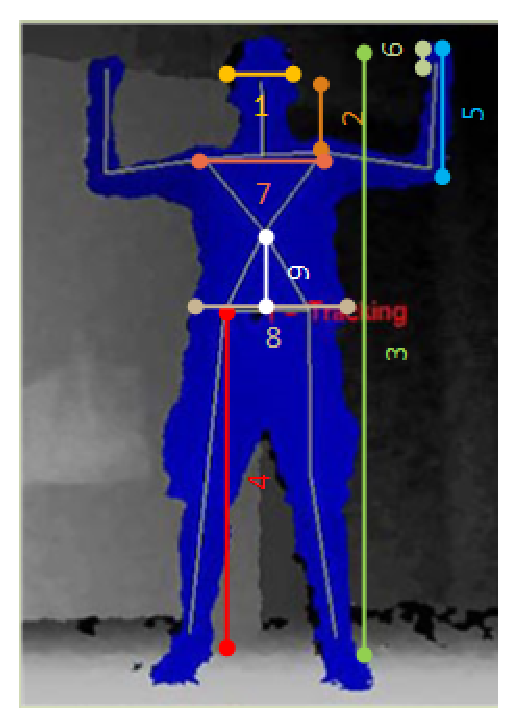
\includegraphics[width=0.9\columnwidth]{./figures/body_proportions.eps}
	\end{center}
	\caption{Human body proportions.}
	\label{fig:body_proportions}
\end{figure}

The measurements are performed in the real-world space, rather than the projective space, because a real size estimation is crucial for determining the appropriate cloth size. The latter would be sufficient for simulation purposes, when there is no concern of real-life apparel fitting. After the acquisition of the required scaling parameters for the subject, the cloth and avatar should be scaled as a whole in three dimensions uniformly, in contrast to a segmented scaling. This decision is based on the scope of our work because it is a standard-sized apparel fitting application without extensive customization. Following the measurements, the body width and shoulder height are estimated as follows:

\begin{enumerate}
\item Take the primary dimension (either the body height or shoulder width) $P_i^0$. This process is repeated for width (W) and height (H).
\item Using the remaining measurements in the set, estimate the primary dimension $P_i$ as $P_i^j$ using proportion $R_i^j$ from \ref{tbl:human_body_proportions}.
\begin{equation}
W,H_i^j=W,H_j \times R_i^j
\label{eqn:proportion_estimation}
\end{equation}
\item Find the optimized primary dimension as the mean of all estimations:
\begin{equation}
W,H_i=\frac{1}{(n+1)} \times \sum\limits_{j=0}^n W,H_i^j
\label{eqn:optimized_parameter}
\end{equation}
\end{enumerate}

\begin{algorithm}
\DontPrintSemicolon 
\KwIn{Human body proportions and the user and depth data}
\KwOut{The body width and shoulder height}
$t_{\textit{proportion}}=import(\mbox{Table}~\ref{tbl:human_body_proportions})$ \;
$t_{\textit{primary}}= (w_{\textit{shoulder}}, \; h_{\textit{body}})$ \;
$ct=cloth_{\textit{type}}$\;
${\textit{width}}_{\textit{main}}=t_{\textit{proportion}}.width(ct)$\;
${\textit{width}}_{\textit{sum}}=0$\;
$count_{\textit{effector}}=0$\;
\ForEach{{\textit{width}} \bf{in} $t_{\textit{proportion}}$ }{
$w_i=measure(p_i)$\;
$w_i^j=w \times t_{\textit{proportion}}.ratio(p_i,\textit{\textit{width}}_{\textit{main}})$\;
${\textit{width}}_{\textit{sum}}=width_{\textit{sum}}+w_i^j $\;
$count_{\textit{effector}}++ $\;
}
${\textit{width}}_{weighted}=\frac{\textit{\textit{width}}_{\textit{sum}}}{\textit{count}_{\textit{effector}}}$\;
$x_s=\frac{\textit{\textit{width}}_{\textit{weighted}}}{\textit{\textit{width}}_{\textit{cloth}}}$\;

${\textit{height}}_{\textit{main}}=t_{\textit{proportion}}.{\textit{height}}(ct)$\;
${\textit{height}}_{\textit{sum}}=0$\;
$count_{effector}=0$\;
\ForEach{{\textit{height}} \bf{in} $t_{\textit{proportion}}$ }{
$h_i=measure(p_i)$\;
$h_i^j=h \times t_{\textit{proportion}}.ratio(p_i,\textit{\textit{height}}_{\textit{main}})$\;
${\textit{height}}_{\textit{sum}}={\textit{height}}_{\textit{sum}}+h_i^j $\;
$count_{\textit{effector}}++ $\;
}
$\textit{\textit{height}}_{\textit{weighted}} = \frac{\textit{\textit{height}}_{\textit{sum}}}{\textit{count}_{\textit{effector}}}$\;
$y_{s}=\frac{\textit{\textit{height}}_{\textit{weighted}}}{\textit{\textit{height}}_{\textit{cloth}}}$\;
\Return{$(x_s, \; y_s)$}
\caption{Body Dimension Estimation}
\label{algo:cloth_resize}
\end{algorithm}

\subsection{Temporal Optimization}
\label{subsec:4�3} 

By now, we have acquired the required body dimensions and collision sphere parameters for a realistic simulation. 
Yet, the measurements are performed on a filtered version of a depth sensor with high error rates. In order to overcome the noise and overall depth-sense faults, the prior measurements are repeated for the duration of one second, which corresponds to 30 frames of input depth map. 
A considerably different approach here would be to employ the temporal averaging on the depth map instead of the measured parameters. We observe that the results suffer due to the motions of the subject because most subjects fails to keep their exact form for one second. To overcome these problems, we use temporal averaging that takes the mean of the specified parameters for the frames in one second. This step finalizes the parameters and delivers the required parameters for simulation environment synthesis. 

\begin{algorithm}
\DontPrintSemicolon % Some LaTeX compilers require you to use \dontprintsemicolon instead
\KwIn{Raw depth stream from the depth sensor}
\KwOut{Final collision sphere radii and body dimensions}
\tcc{s is a buffer for storing x and y scaling parameters for 30 frames}
\tcc{r is a buffer for storing for collision sphere radii of 16 joints for 30 frames}
float s[30, 2], r[30, 16] \;
\For{i \bf{from} 0 \bf{to} $30 frames$ }{
	r[i][1:16]=fitSpheres()\;
	s[i][1:2]=optimizeScaleParameters()\;
}
$r_{\textit{final}}$  = \textrm{avg}(r)\;
$s_{\textit{final}}$  = \textrm{avg}(s)\;
\caption{Temporal Averaging}
\label{algo:temporal_averaging}
\end{algorithm}


\section{Motion Smoothing}
\label{sec:Motion}
Our framework utilizes a virtual 3d avatar to display and simulate the apparel models. The avatar imitates the motions of the actual user, using the orientation data acquired from the depth sensor middleware. However, application of the raw data from the sensor causes unnatural movements due to the noise in the sensor input, self-occlusions of the body and inadequate IK solvers.  In order to present a more realistic avatar animation, a series of filters and constraints are applied to the sensor data. 

\subsection{Position Filtering}
The most severe disruption of the self-occlusion problem takes place in the joint position acquisition. There is no possible way of acquiring the correct position of a limb when the sensor has no vision of it. However, the way humans move their limbs under normal conditions follow certain principles and trends which can be used to estimate the locations of occluded body parts. The nature of these motions, demonstrating traits similar to seasonal behavior make them suitable for a variety of filters\cite{Azimi2012}. We decided to go with the Holt-Winters Double Exponential smoothing \cite{Kalekar2004} as it comes with the middleware, easy to use and delivers good quality results with acceptable latency for the purposes of this application. 

\subsection{Rotation Filtering and Constraints}
The joint orientations are acquired from the sensor middleware directly, however the data is not smooth. Although the middleware enforces certain constraints (such as allowing only pitch rotations on Ulna), there are often significant gaps in the estimated angles which produce unnatural tremor-like movements on the avatar. Furthermore, there is no filtering of unnatural rotations which take place when an occluded body part is estimated to be in a wrong location. 

\begin{figure*}
	\centerline{
	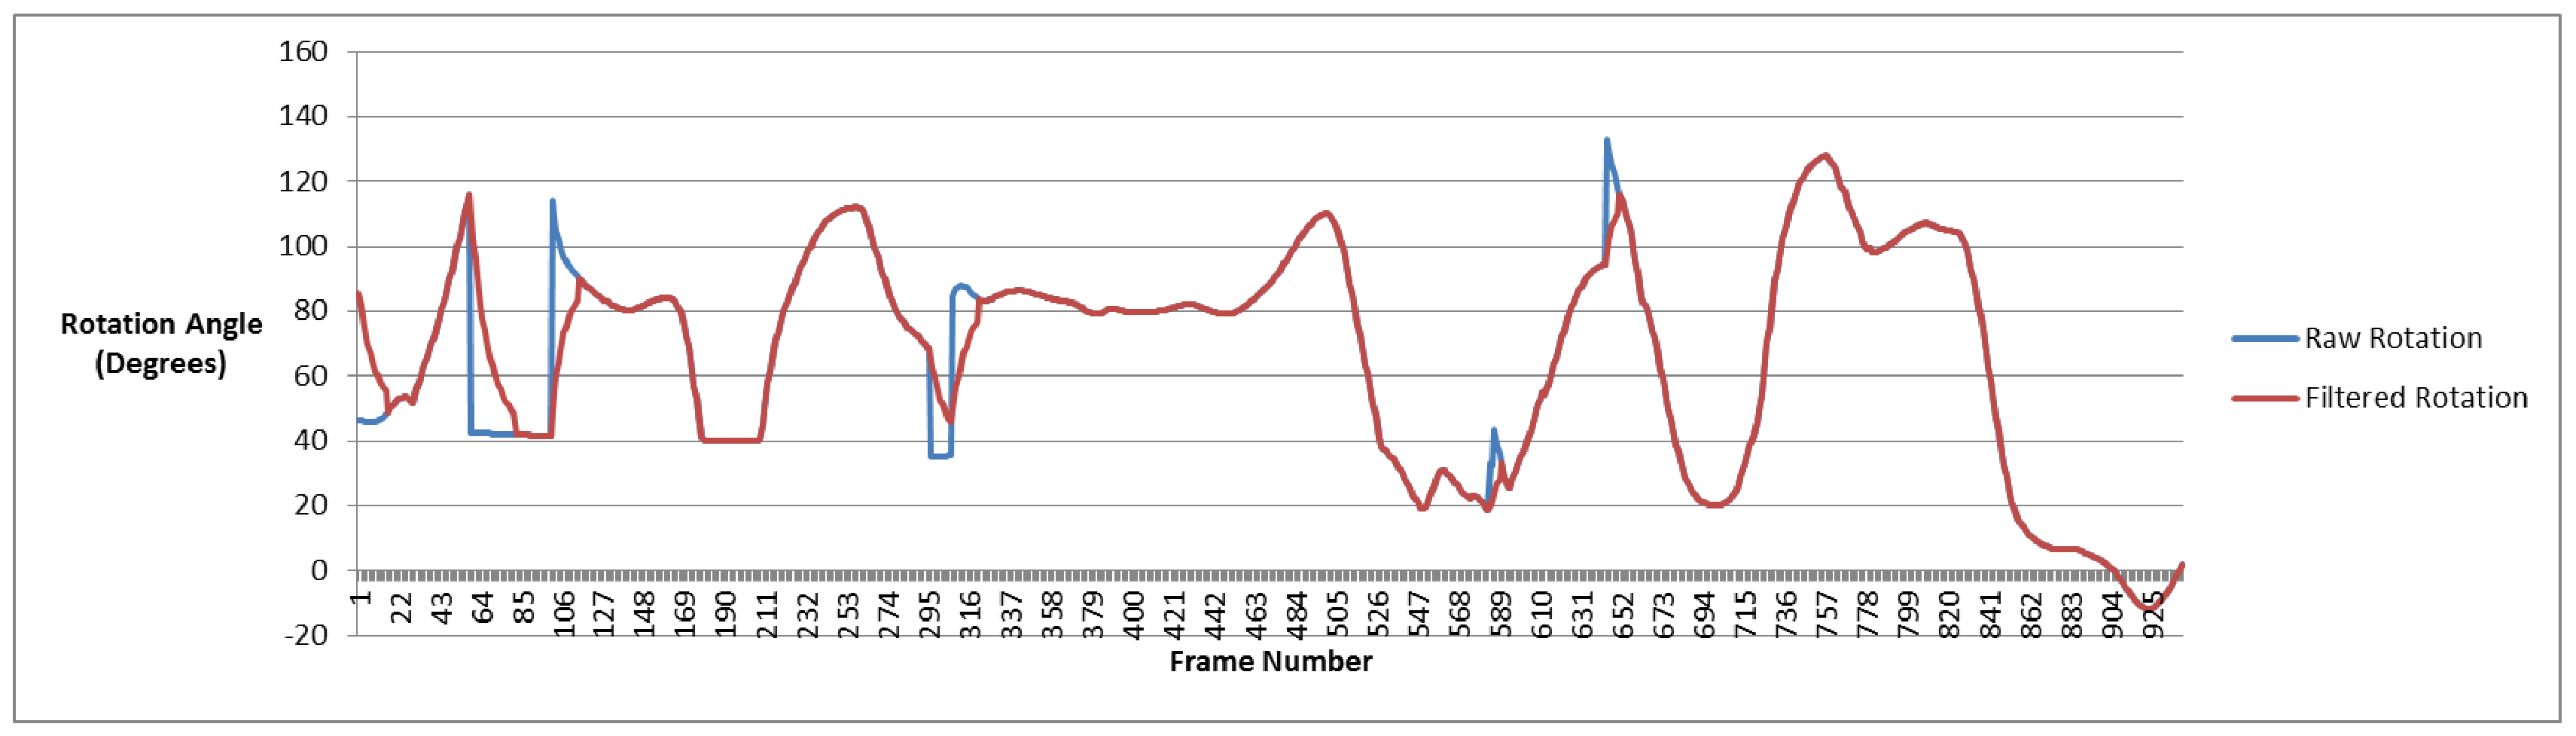
\includegraphics[width=2.0\columnwidth]{./figures/rotation-filter.eps}
	}
\caption{The row and filtered samples for Right Humerus Roll Angle}
	\label{fig:rotation-filter}
\end{figure*}

The inferior quality of the orientation data is improved in two stages: applying another set of constraints on the joint data based on the natural limits of human bones, followed by as asymptotic smoothing of the joint angles to prevent the effect of gaps in the angles-see Figure\ref{fig:rotation-filter}. 

\subsection{Bone Splitting}
The lower sections of human limbs contain two parallel bones allowing the twisting rotation on the hands and feet. The configuration of bones allow all portions of the lower limb follow the bones in pitch and roll rotations, although the effect of yaw rotation decreases as it gets closer to the mid-section joint (elbow or knee). This effect is not possible to achieve with a single bone fore-arm representation, as specified in the highest level of detail in the H-ANIM standard \cite{HANIM}, using unified weights (same for all types of rotations, transformations and scaling) and linear skinning. On the other hand, applying a different set of weights for each possible transformation, rotation or scaling requires additional space and time which can be considered redundant as it is not going to be used in most of the skeleton and mesh and not implemented in most of the popular rendering engines. This problem is previously addressed by Kavan et. al\cite{Kavan2009}, proposing a method of introducing additional blending bones to simulate non-linear skinning, however the generalized approach is not suitable for a real time application with previously unknown motions. 

As our only problematic bones for this particular case is the upper limbs, we employed a novel approach to solve this problem by introducing an additional bone connected in series for the upper limbs. The Humerus and Ulna bones are split halfway and the lower sections are labeled as Humerus-Extension and Ulna-Extension respectively. The vertex weights in the corresponding sections are divided linearly among two sections as seen in Figure \ref{fig:forearm-weights}. 

\begin{figure} 
	\begin{center}
	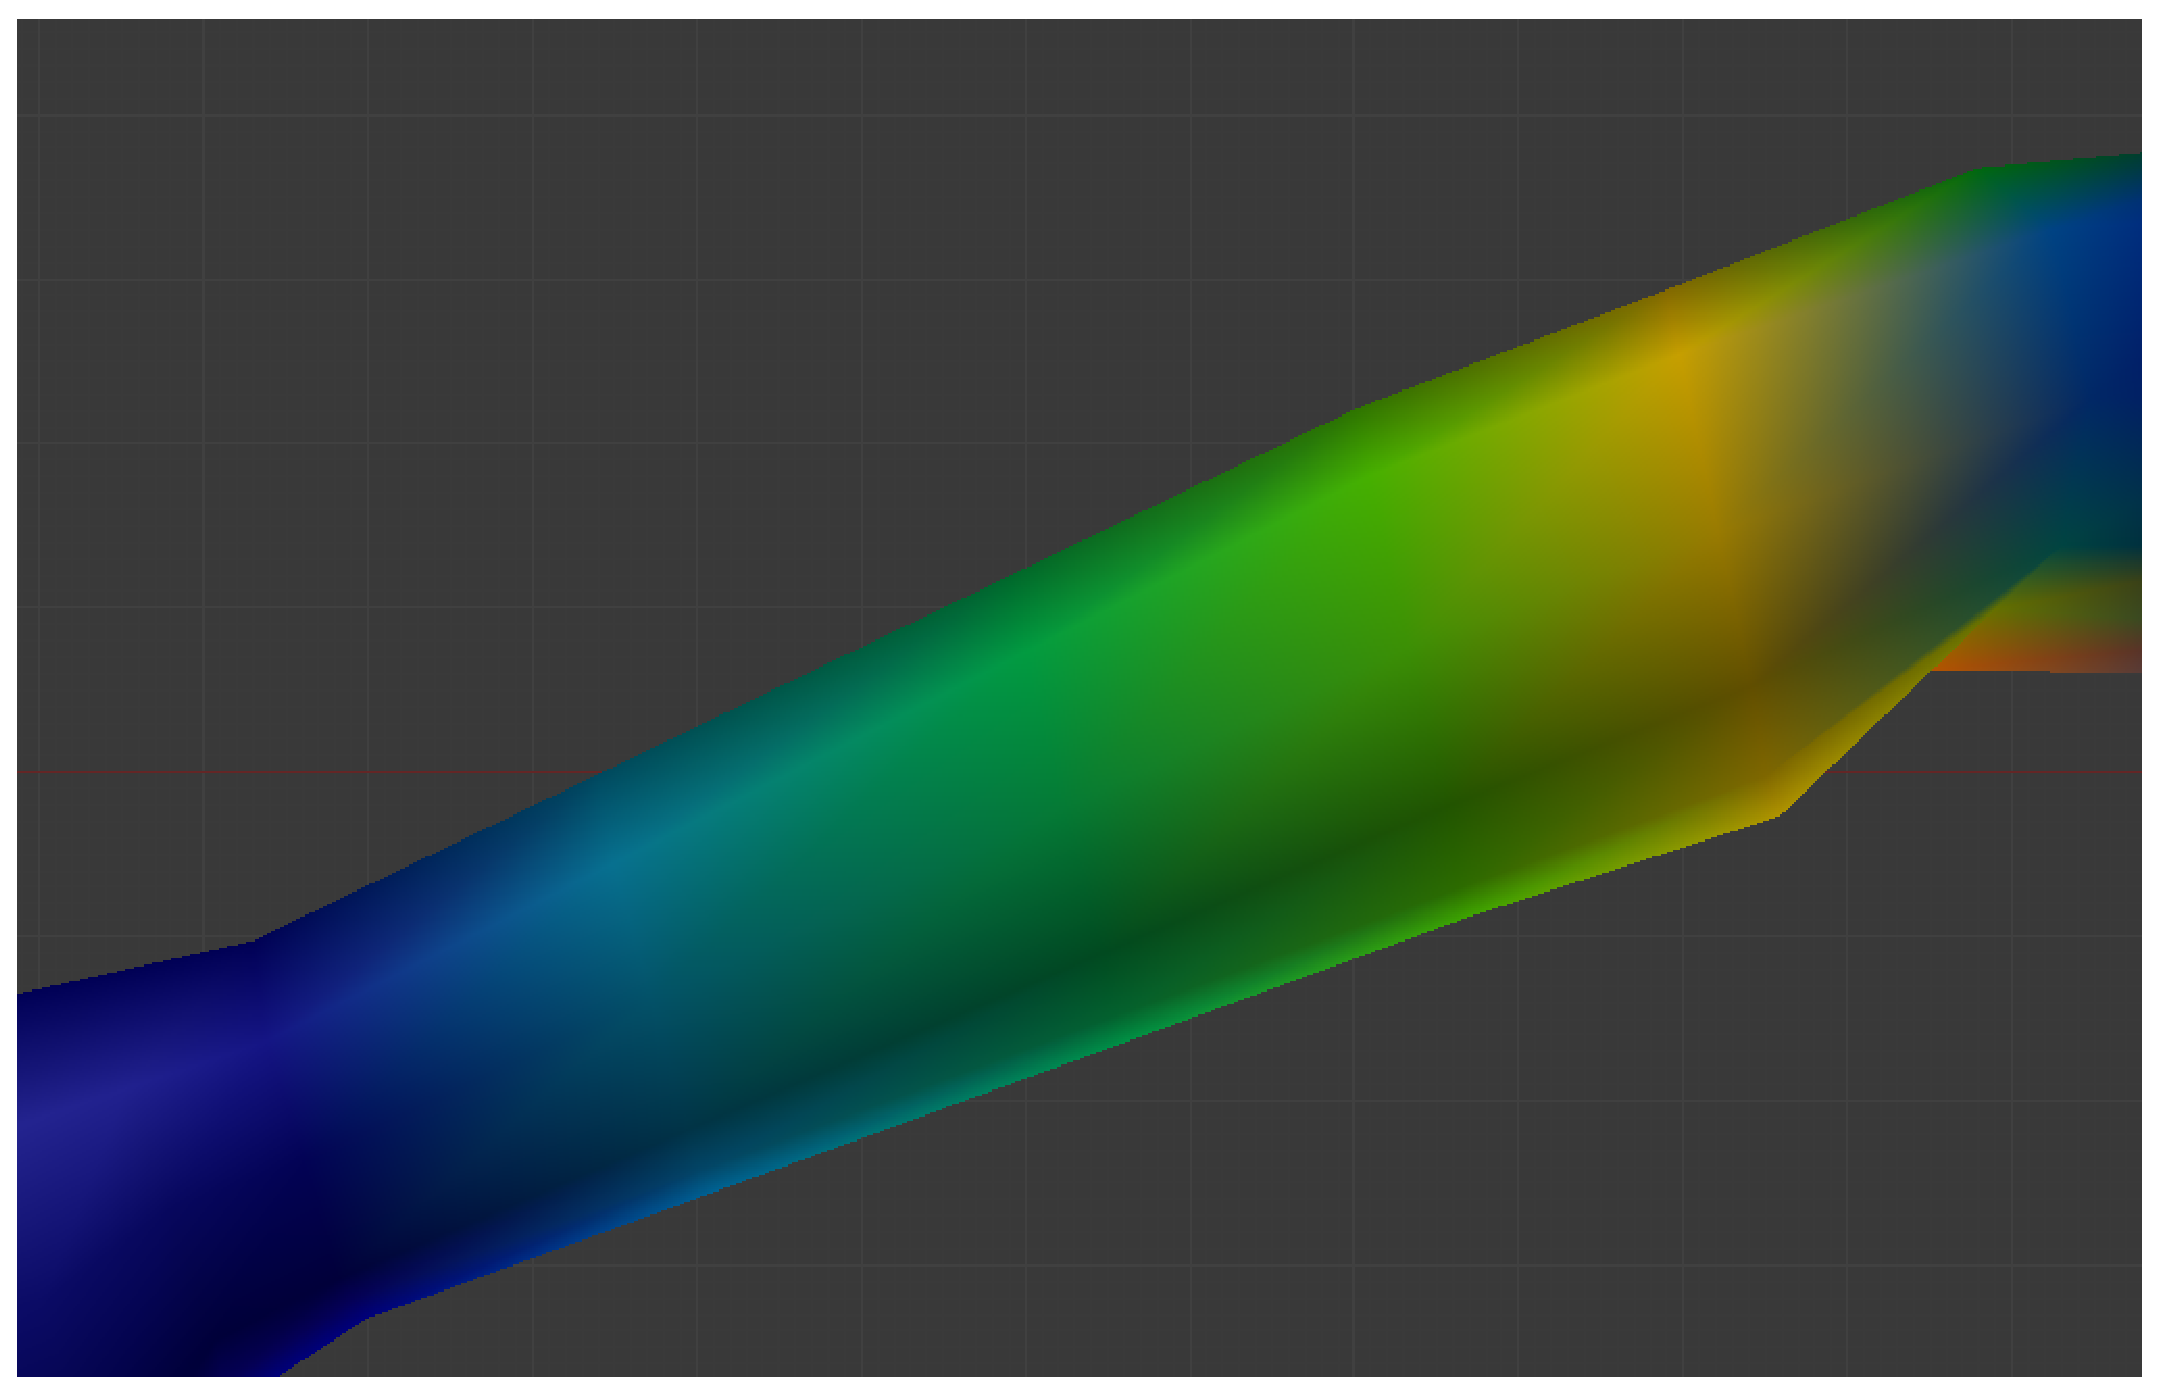
\includegraphics[width=1.0\columnwidth]{./figures/ulna-weight.eps}
	(a)
	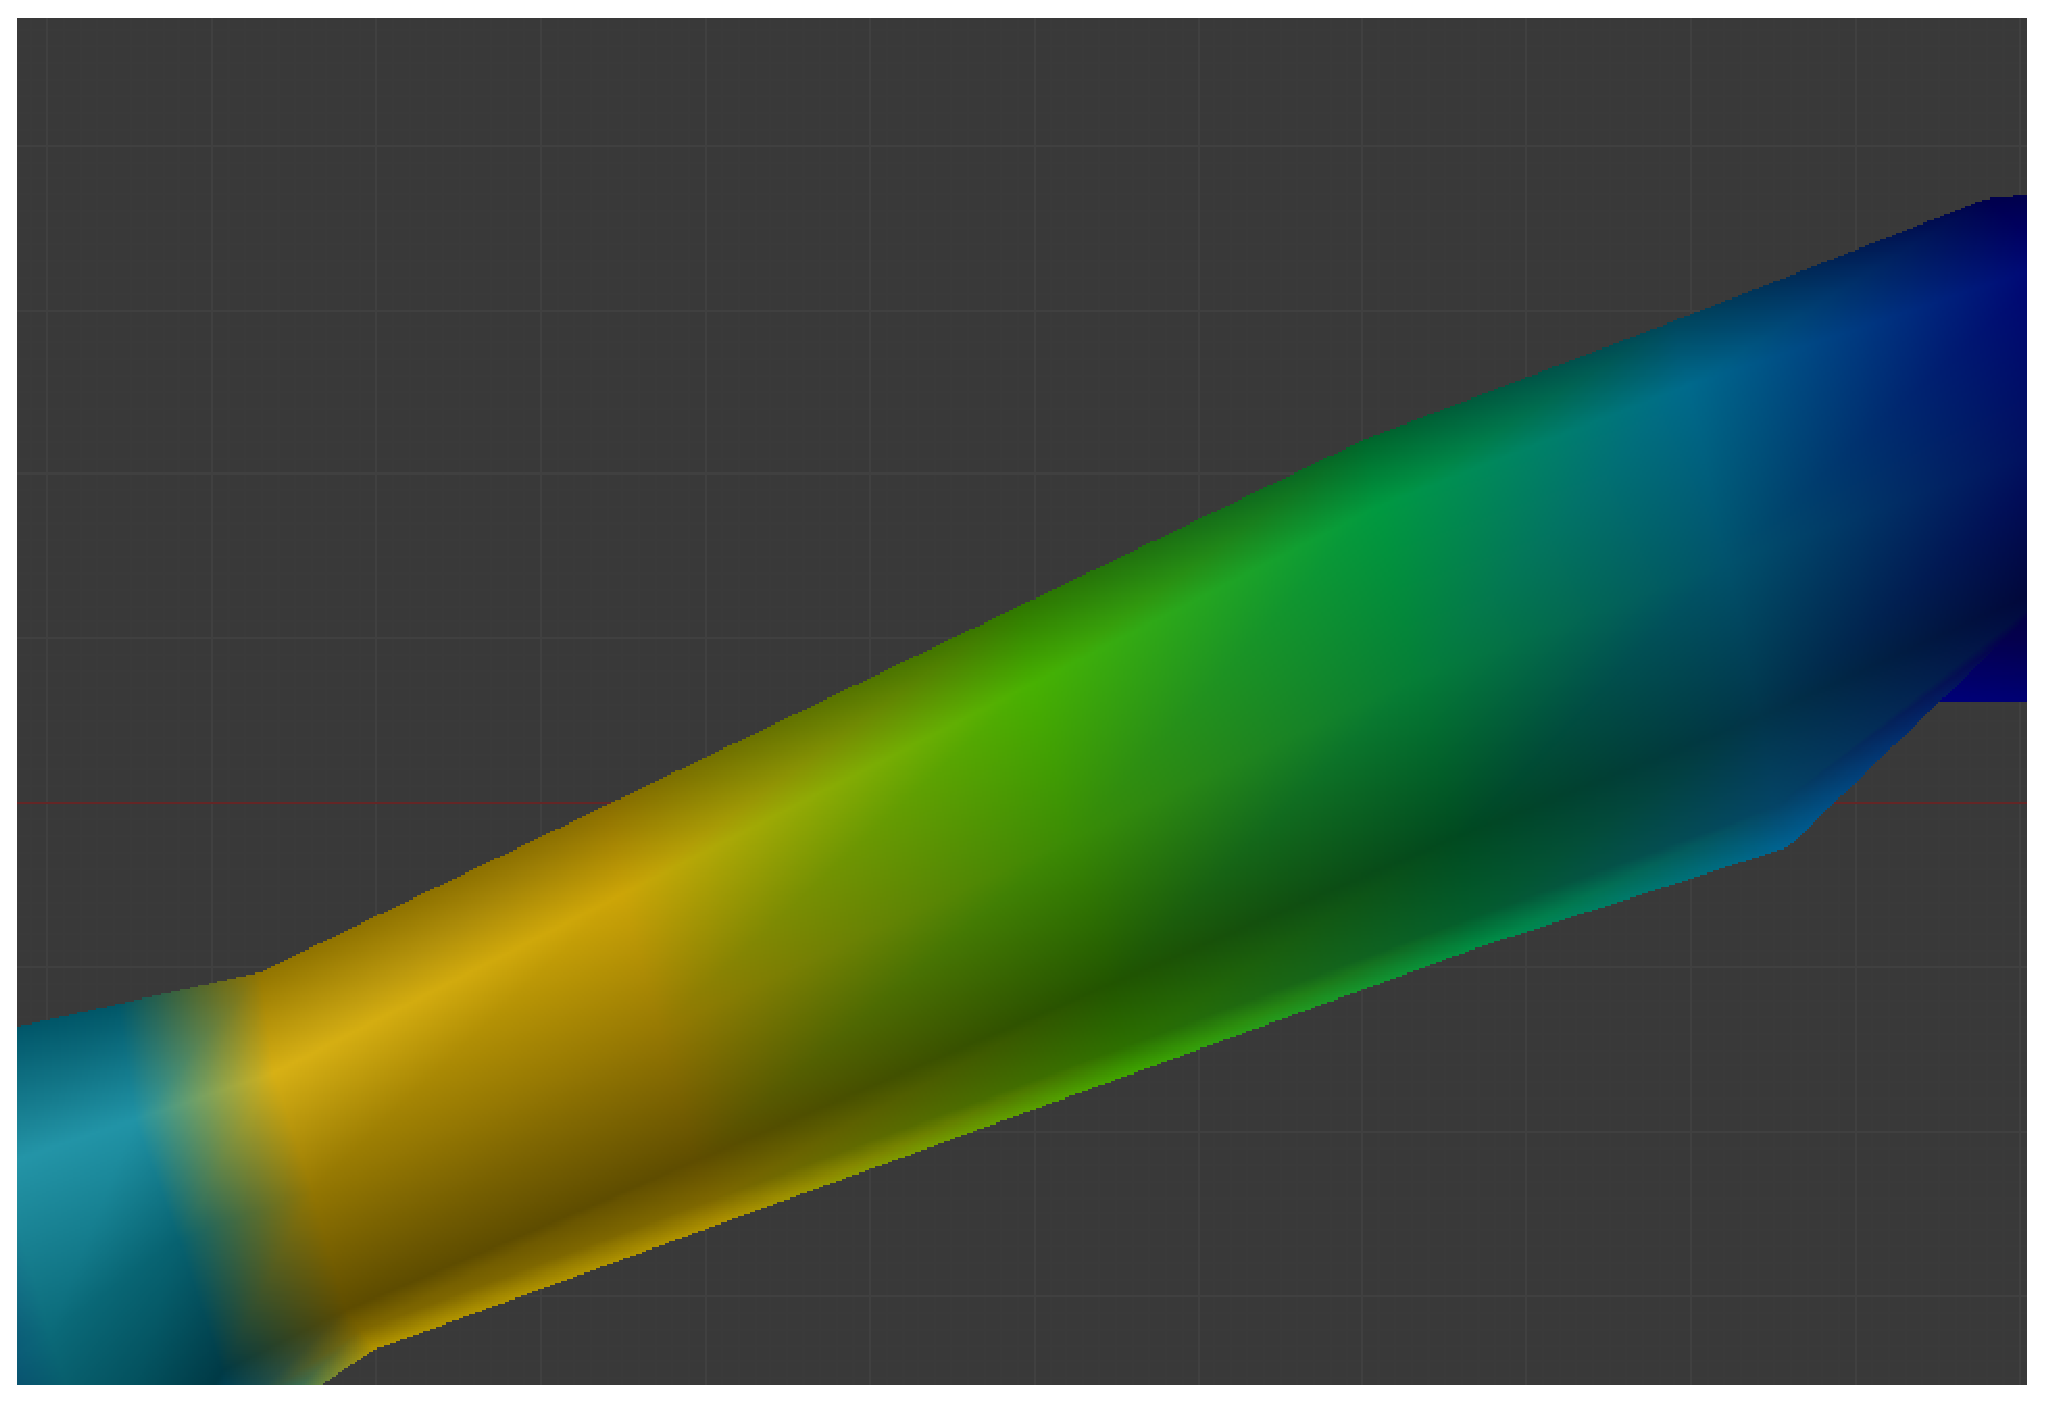
\includegraphics[width=1.0\columnwidth]{./figures/ulna-extent-weight.eps}
	(b)
	\end{center}
	\caption{The vertex weights for: (a) upper ulna and (b) lower ulna bone.}
	\label{fig:forearm-weights}
\end{figure}


During runtime, the filtered local rotation of the upper limb bones are separated into two distinct rotations, one containing the yaw and the other containing pitch and roll rotations, which are applied to the extension bone and the original bone respectively. With proper weights, the rotation of the users arm is transferred to the virtual avatar naturally without introducing any artifacts. As seen in Figure \ref{fig:forearm-comparison}, the vertices on the forearm twist in a more natural way resembling the real motion.


\begin{figure}
	\begin{center}
	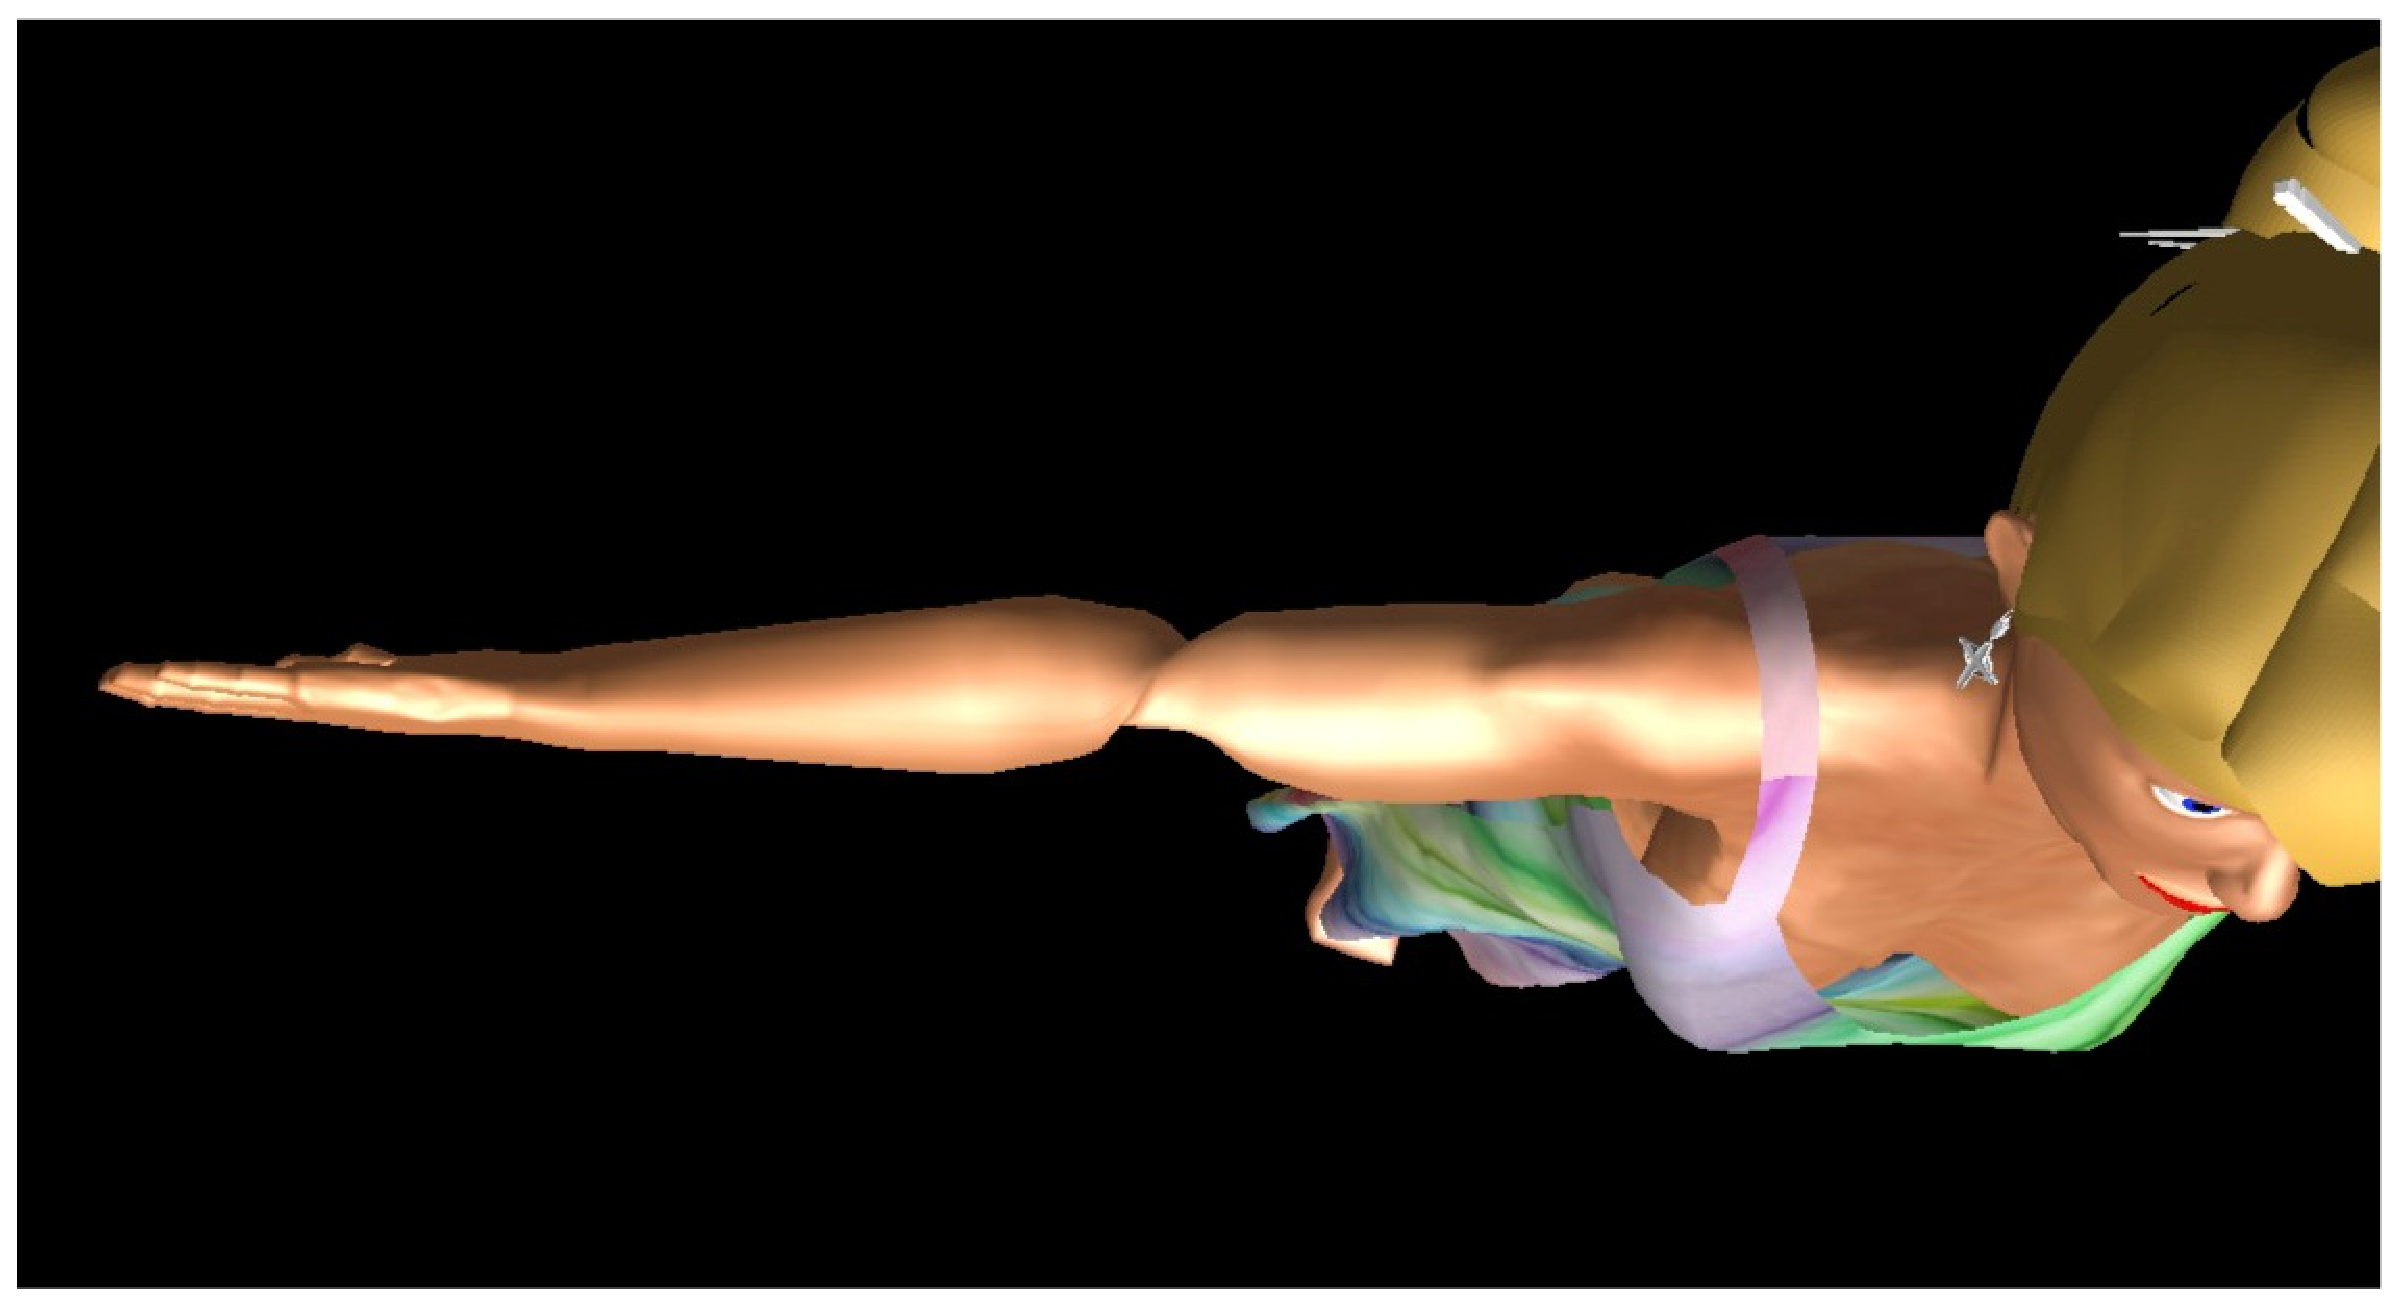
\includegraphics[width=1.0\columnwidth]{./figures/fore-arm-single-bone.eps}
	(a)
	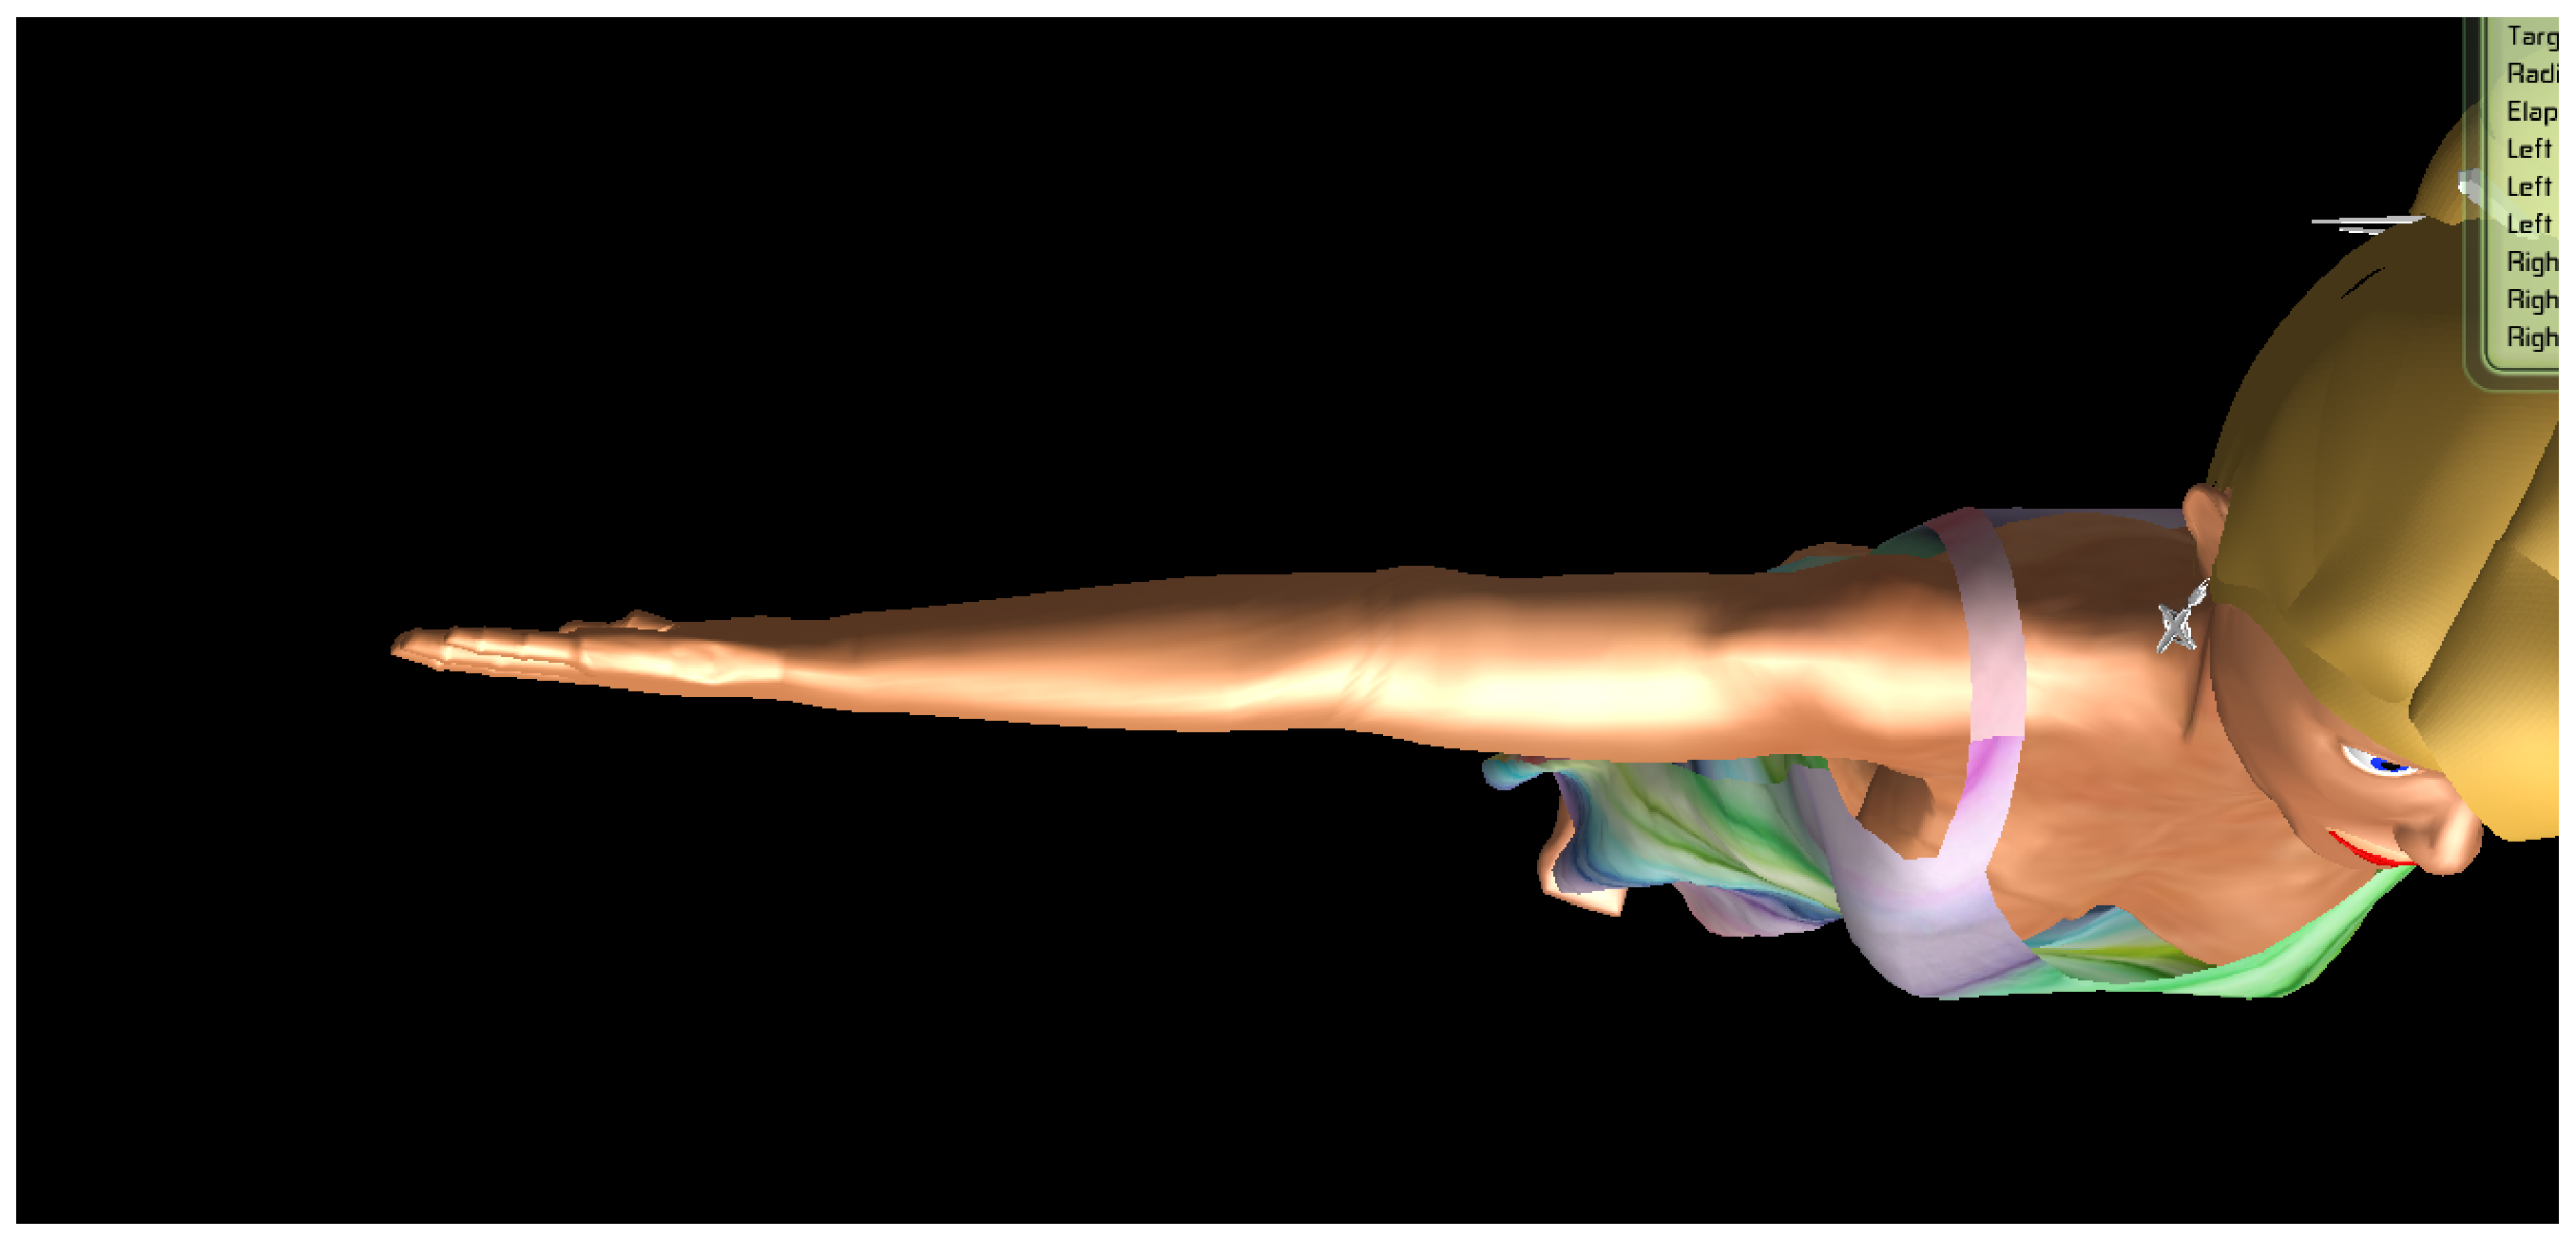
\includegraphics[width=1.0\columnwidth]{./figures/fore-arm-double-bone.eps}
	(b)
	\end{center}
	\caption{Comparison of a -90$^\circ$ yaw rotation on the forearm with: (a) single and (b) double boned skinning.}
	\label{fig:forearm-comparison}
\end{figure}



\section{Experiments}
\label{sec:Experiments}
The optimization algorithm described in Section~~\ref{sec:3} is implemented on the in-house developed virtual dressing framework, which acts as the test bench for experimentation. 

The measurement process runs after a subject is recognized, identified and calibrated for tracking. Following the parameter estimation, the virtual avatar and cloth are created and the simulation starts.

Table~\ref{tbl:body_results} presents the measurements of the body dimensions, as well as the errors and the standard deviations of the measurements in 30 frames for three subjects. Our results are compared with results from \cite{Giovanni2012}, which is also a real-time application, in Table \ref{tbl:performance_compare}.

\begin{table}
\begin{center}
\begin{tabular}{|c|c|c|c|c|c|c|c|c|}
\hline
  & \multicolumn{4}{c|}{\textbf{Shoulder Width (cm)}} & \multicolumn{4}{c|}{\textbf{Body Height (cm)}} \\ \hline
  \rotatebox{90}{Subject } & \rotatebox{90}{Real } & \rotatebox{90}{Estimated } & \rotatebox{90}{Error (\%)} & \rotatebox{90}{Deviation } & \rotatebox{90}{Real } & \rotatebox{90}{Estimated } & \rotatebox{90}{Error (\%)} & \rotatebox{90}{Deviation } \\ \hline
 1 & 43 & 43.6 & 1 & 7.8 & 172 & 170.8 & 0.6 & 2.5  \\ \hline
 2 & 46 & 44.3 & 3 & 8.5 & 176 & 172.1 & 2 & 1.4  \\ \hline
 3 & 51 & 48.8 & 4 & 12.1 & 176 & 174.0 & 1 & 6.6  \\ \hline
 4 & 48 & 50.0 & 4 & 2.5 & 188 & 191.0 & 1.5 & 7.1  \\ \hline
 5 & 44 & 42.6 & 3 & 4.2 & 178 & 175.8 & 1.2 & 3.1  \\ \hline
\end{tabular}
\end{center}
\caption{Performance figures for the three subjects.}
\label{tbl:body_results}
\end{table} 



\begin{table}
\begin{center}
\begin{tabular}{|c|c|c|c|c|} 
\hline 
  & \rotatebox{90}{Error Average} & \rotatebox{90}{Error Deviation} & \rotatebox{90}{Duration} & \rotatebox{90}{Estimation} \\ \hline
  Our Approach & 2.13 \%  & 1.2 \%  & 1 & Fixed \\ \hline 
  Giovanni et al.\cite{Giovanni2012}  & 4 \% & 3 \% & 1 & None \\ \hline
  Samejima et al.\cite{Samejima2012}  & 6.72 \% & 4.68 \% & n/a & PCA \\ \hline
\end{tabular}
\end{center}
\caption{Performance comparison with \cite{Giovanni2012,Samejima2012} regarding height measurements.}
\label{tbl:performance_compare}
\end{table} 
The total time for the measurement algorithm do not exceed 1.005 seconds in any of the cases. Considering 1.0 seconds is the time for acquiring 30 frames of input from the depth sensor, it is safe to say that the proposed algorithm does not introduce any delays and problems for a real time application because it needs to run only once in the beginning of the simulation.

For the collision spheres, the quality of the results can be assessed by the smoothness of the collision simulation, as seen in Figure \ref{fig:system}. Throughout the simulation, unnatural intersections between the cloth and the avatar never take place, while the cloth appears to rest on the skin naturally, without space between the two meshes. Figure~\ref{fig:examples} shows examples of two dresses on a model with different postures generated with our implementation. 

\begin{figure}
	\begin{center} 
			
\includegraphics[width=1.0\columnwidth]{./figures/scshot.eps}
	\end{center}
	\caption{An example depth map data and the corresponding posture of the subject with a virtual cloth on it.}
	\label{fig:system}
\end{figure}
 
\begin{figure*} 
	\centerline{
	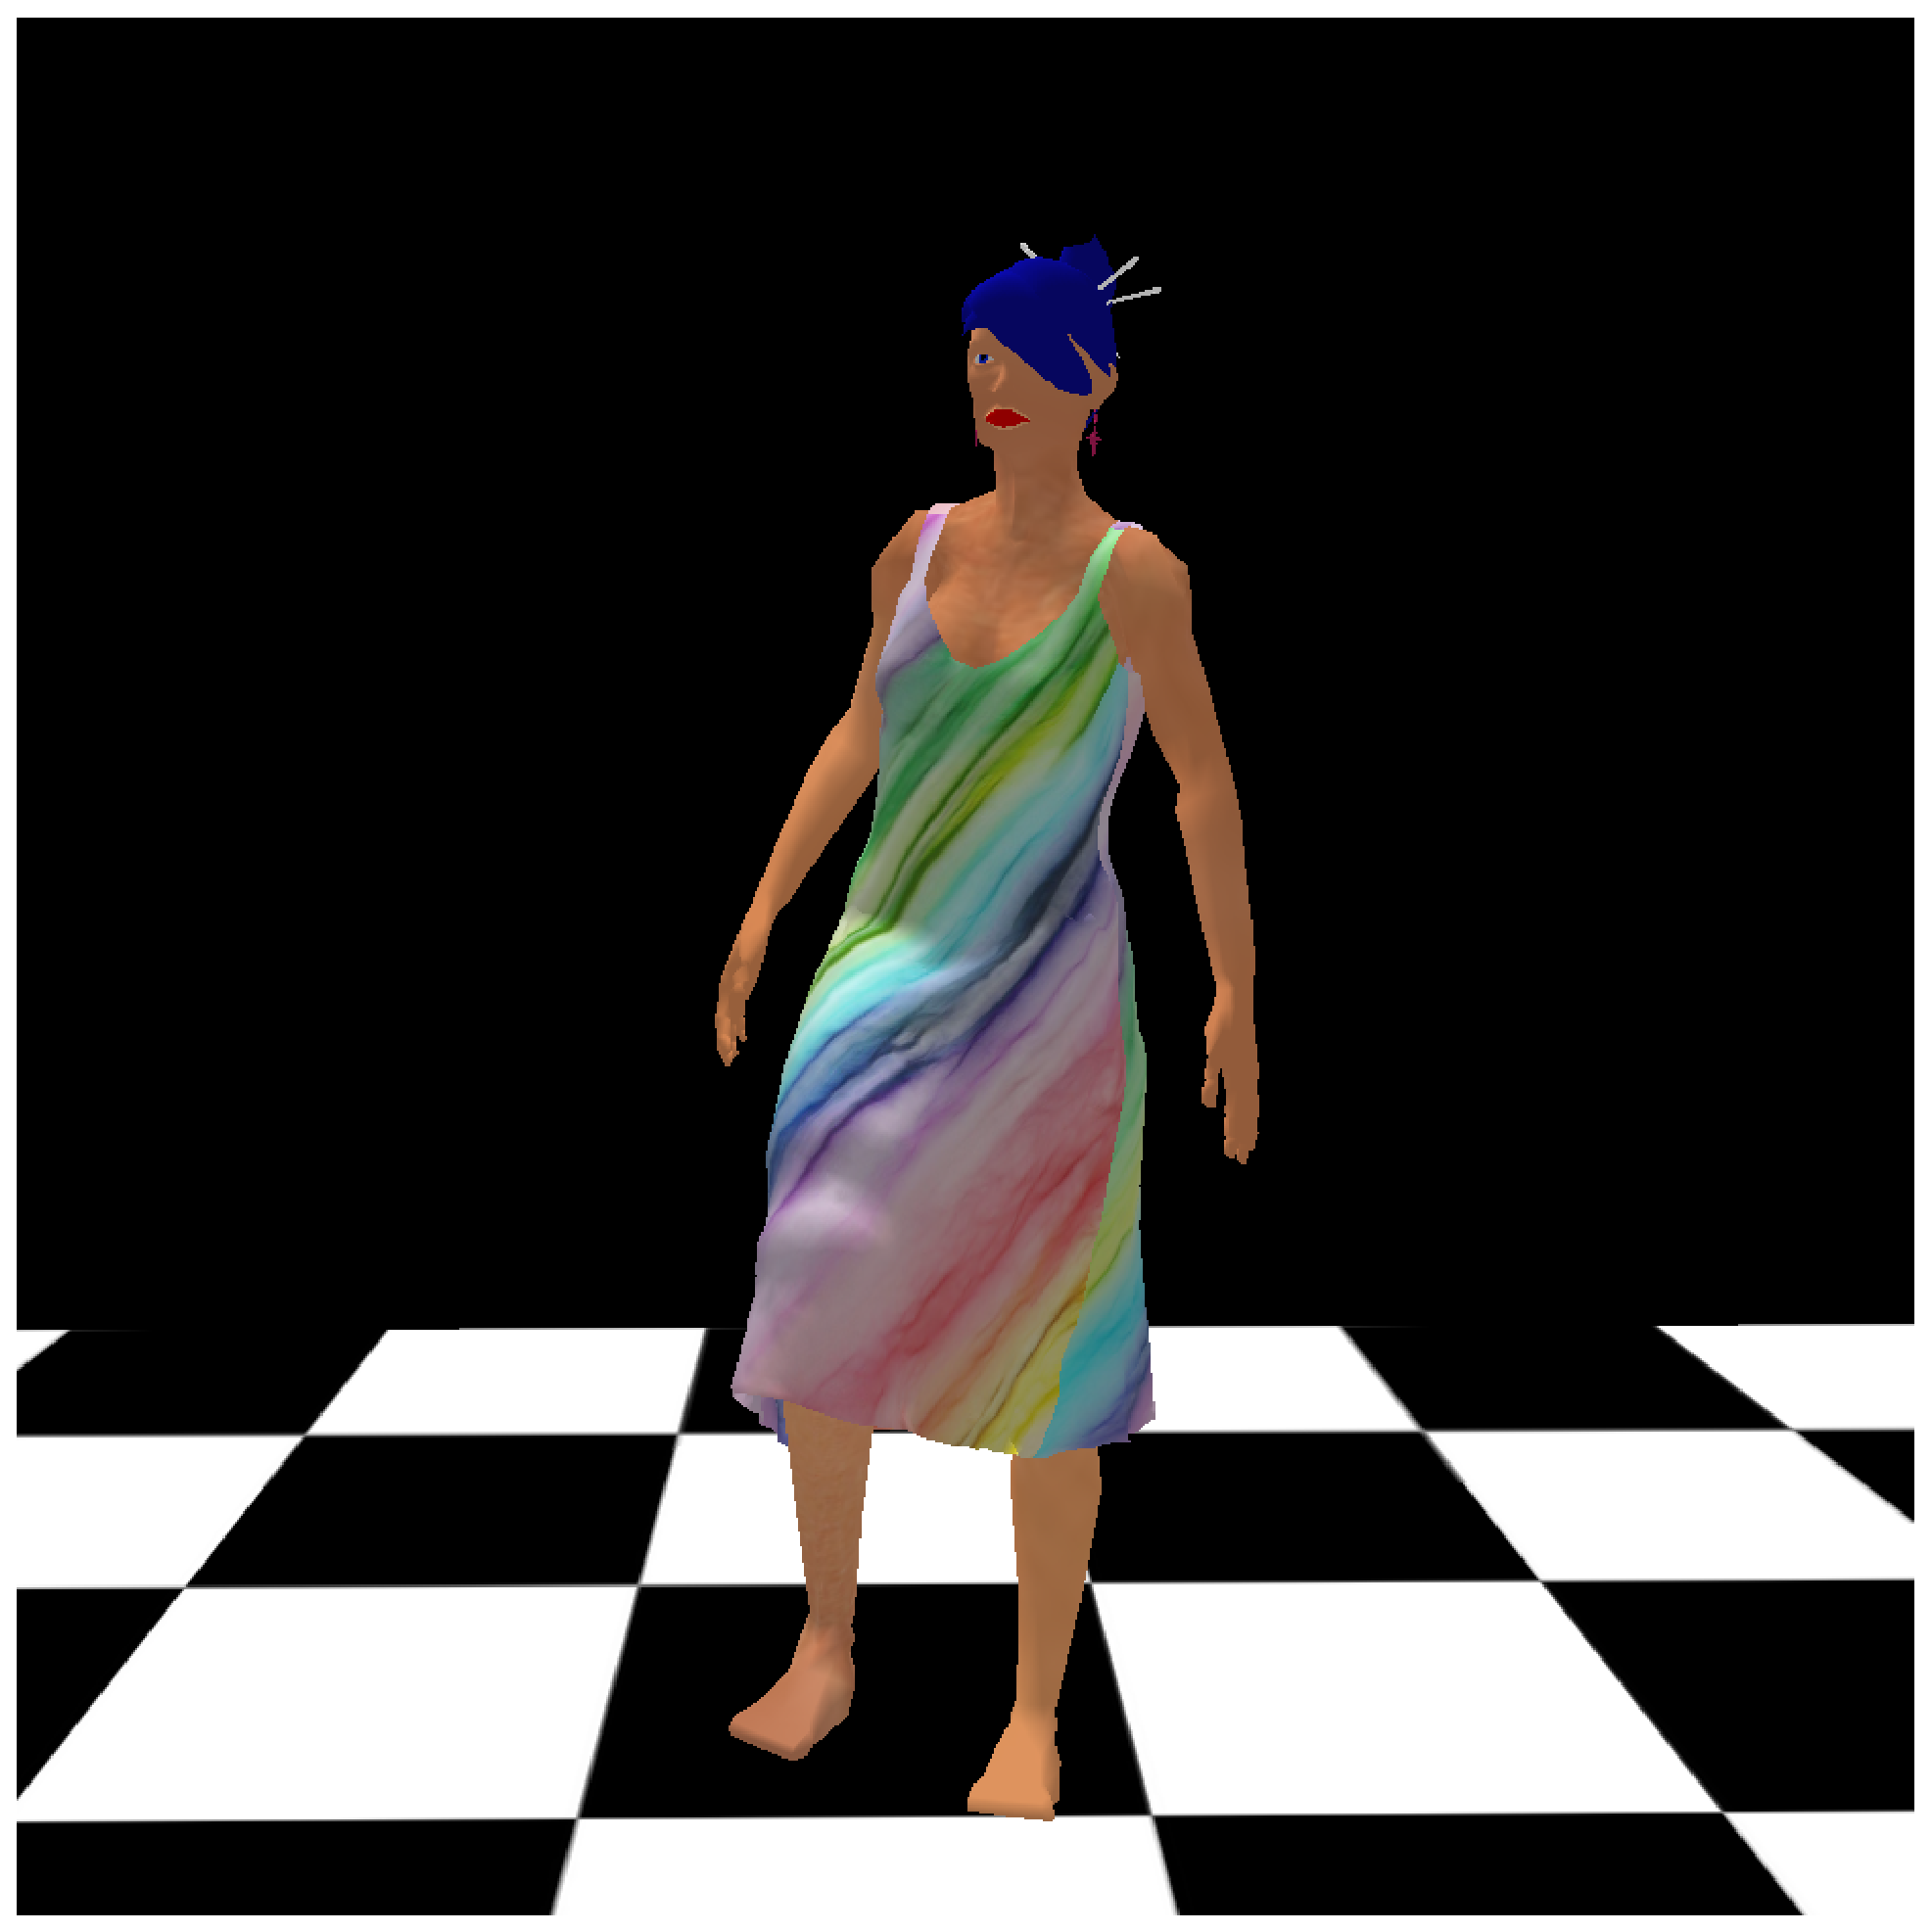
\includegraphics[width=0.50\columnwidth]{./figures/sundress-1.eps}
	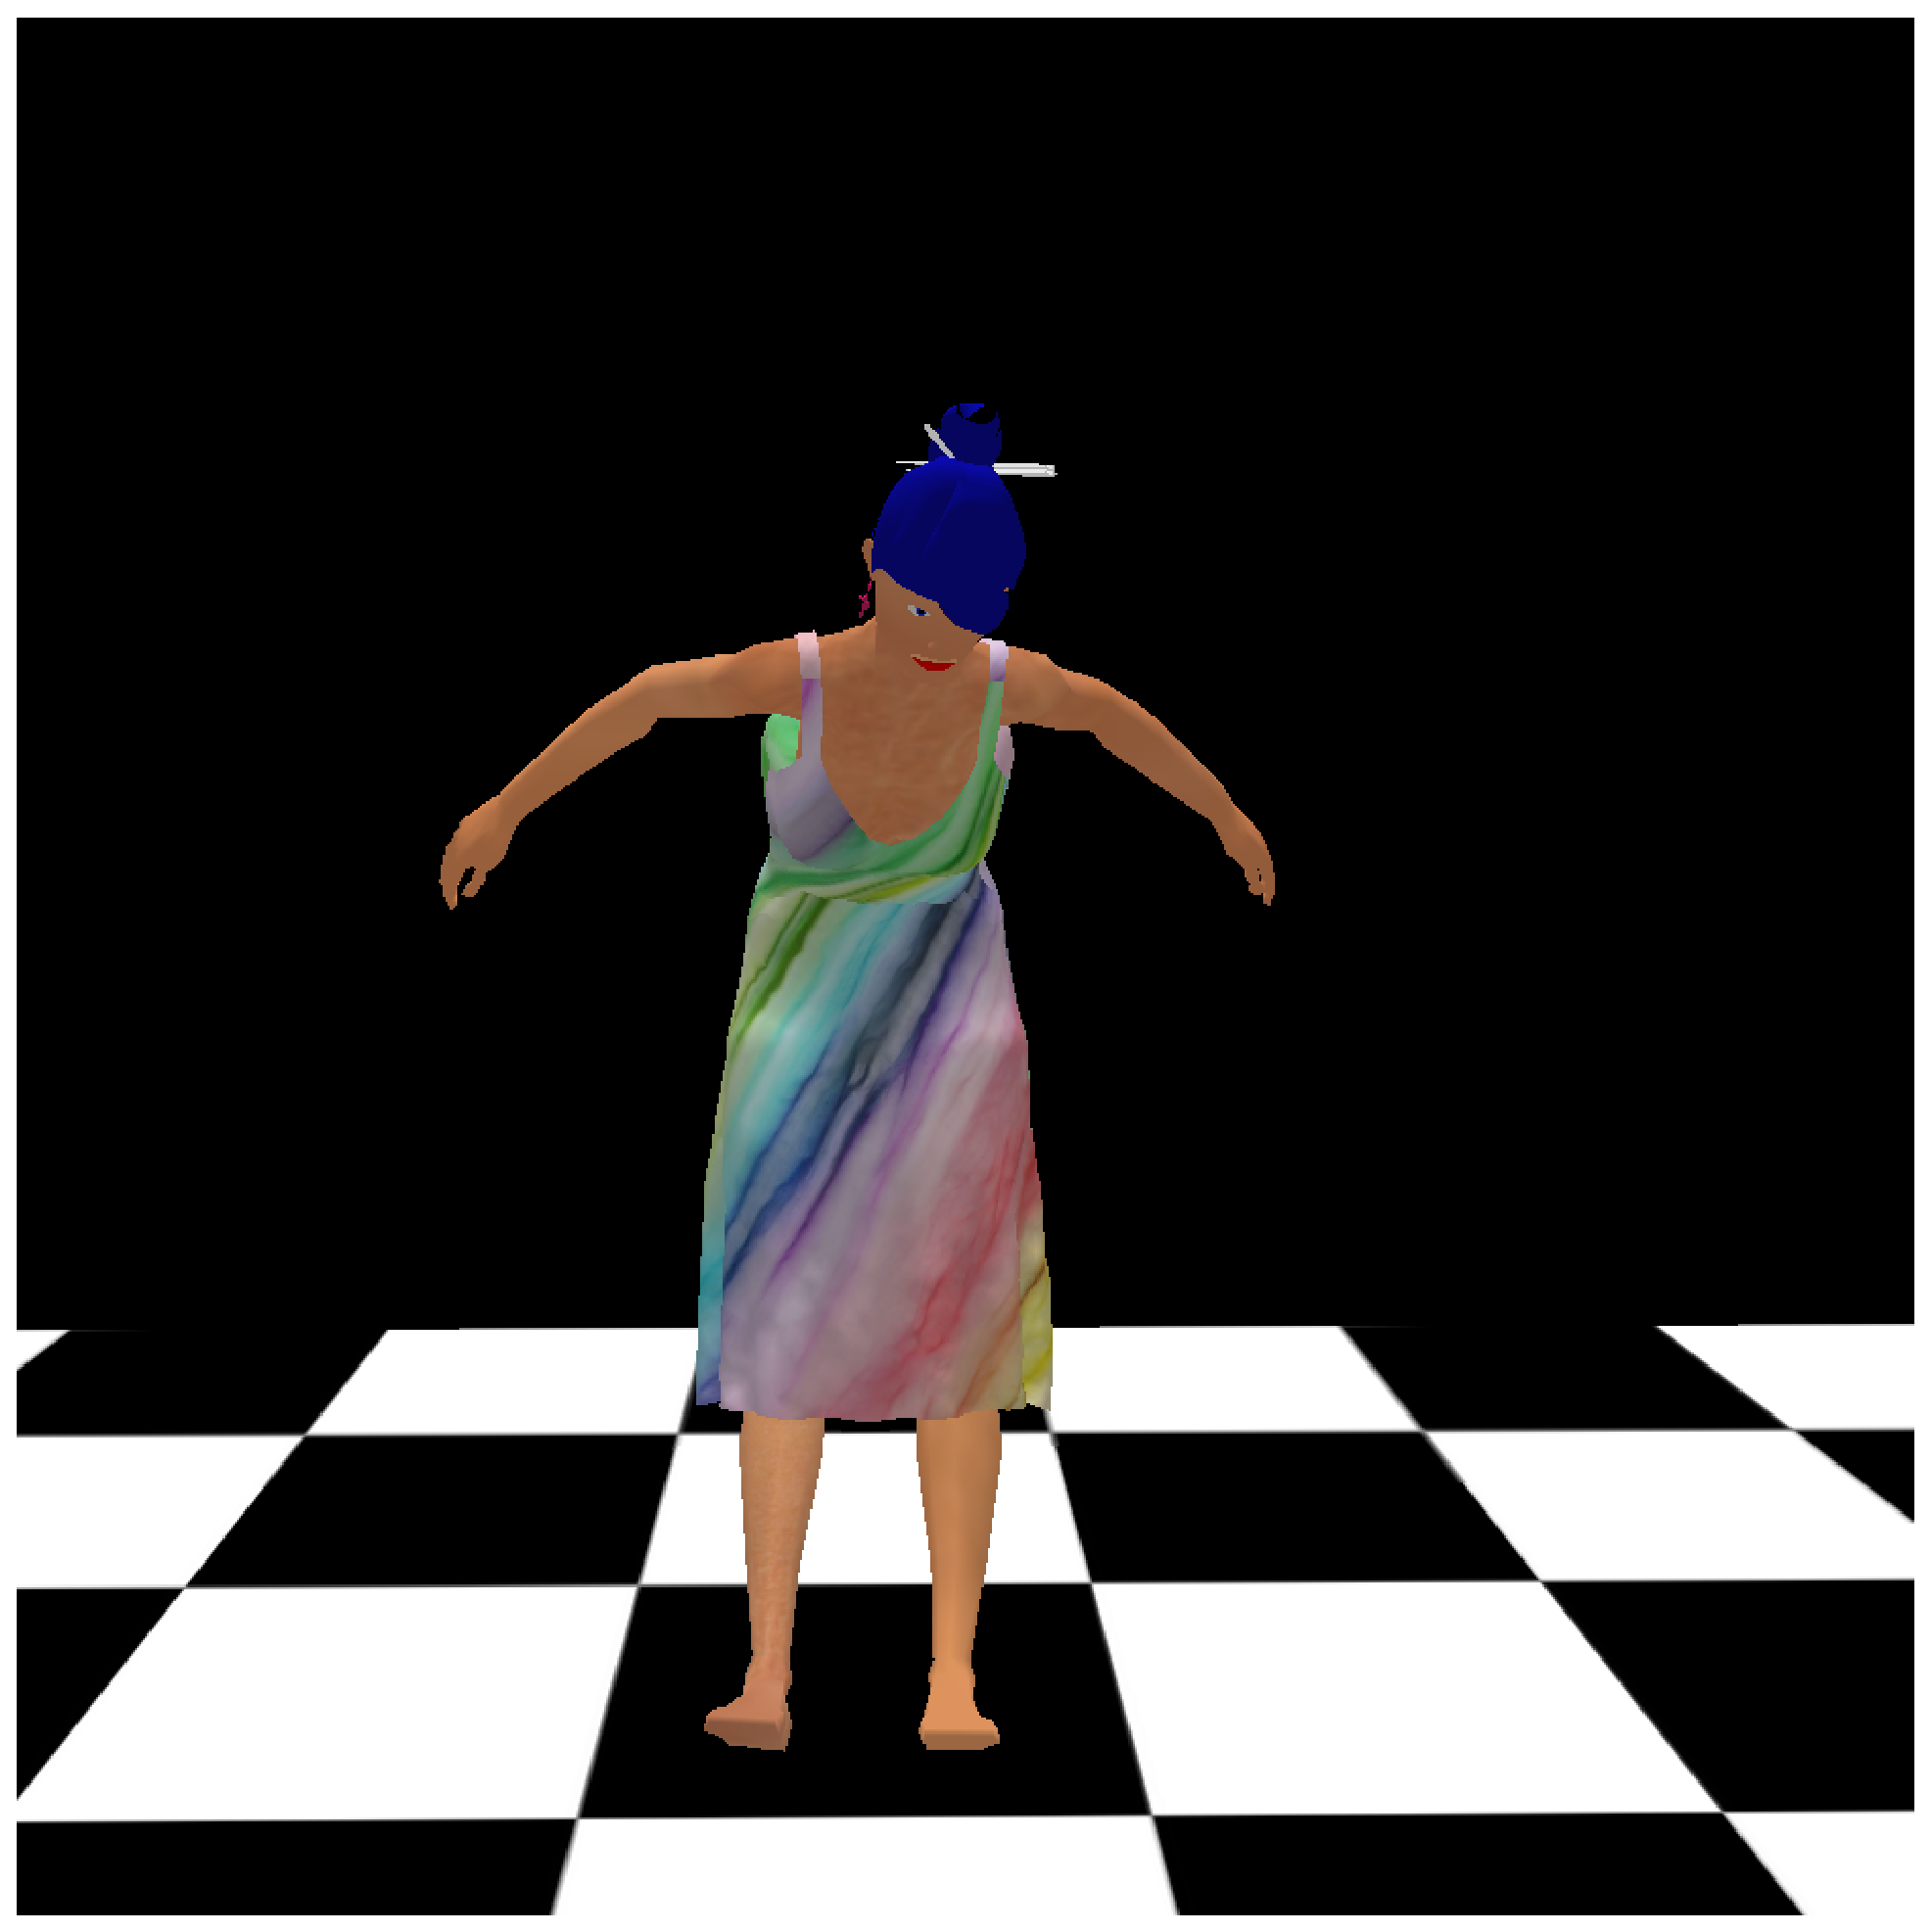
\includegraphics[width=0.50\columnwidth]{./figures/sundress-2.eps}
	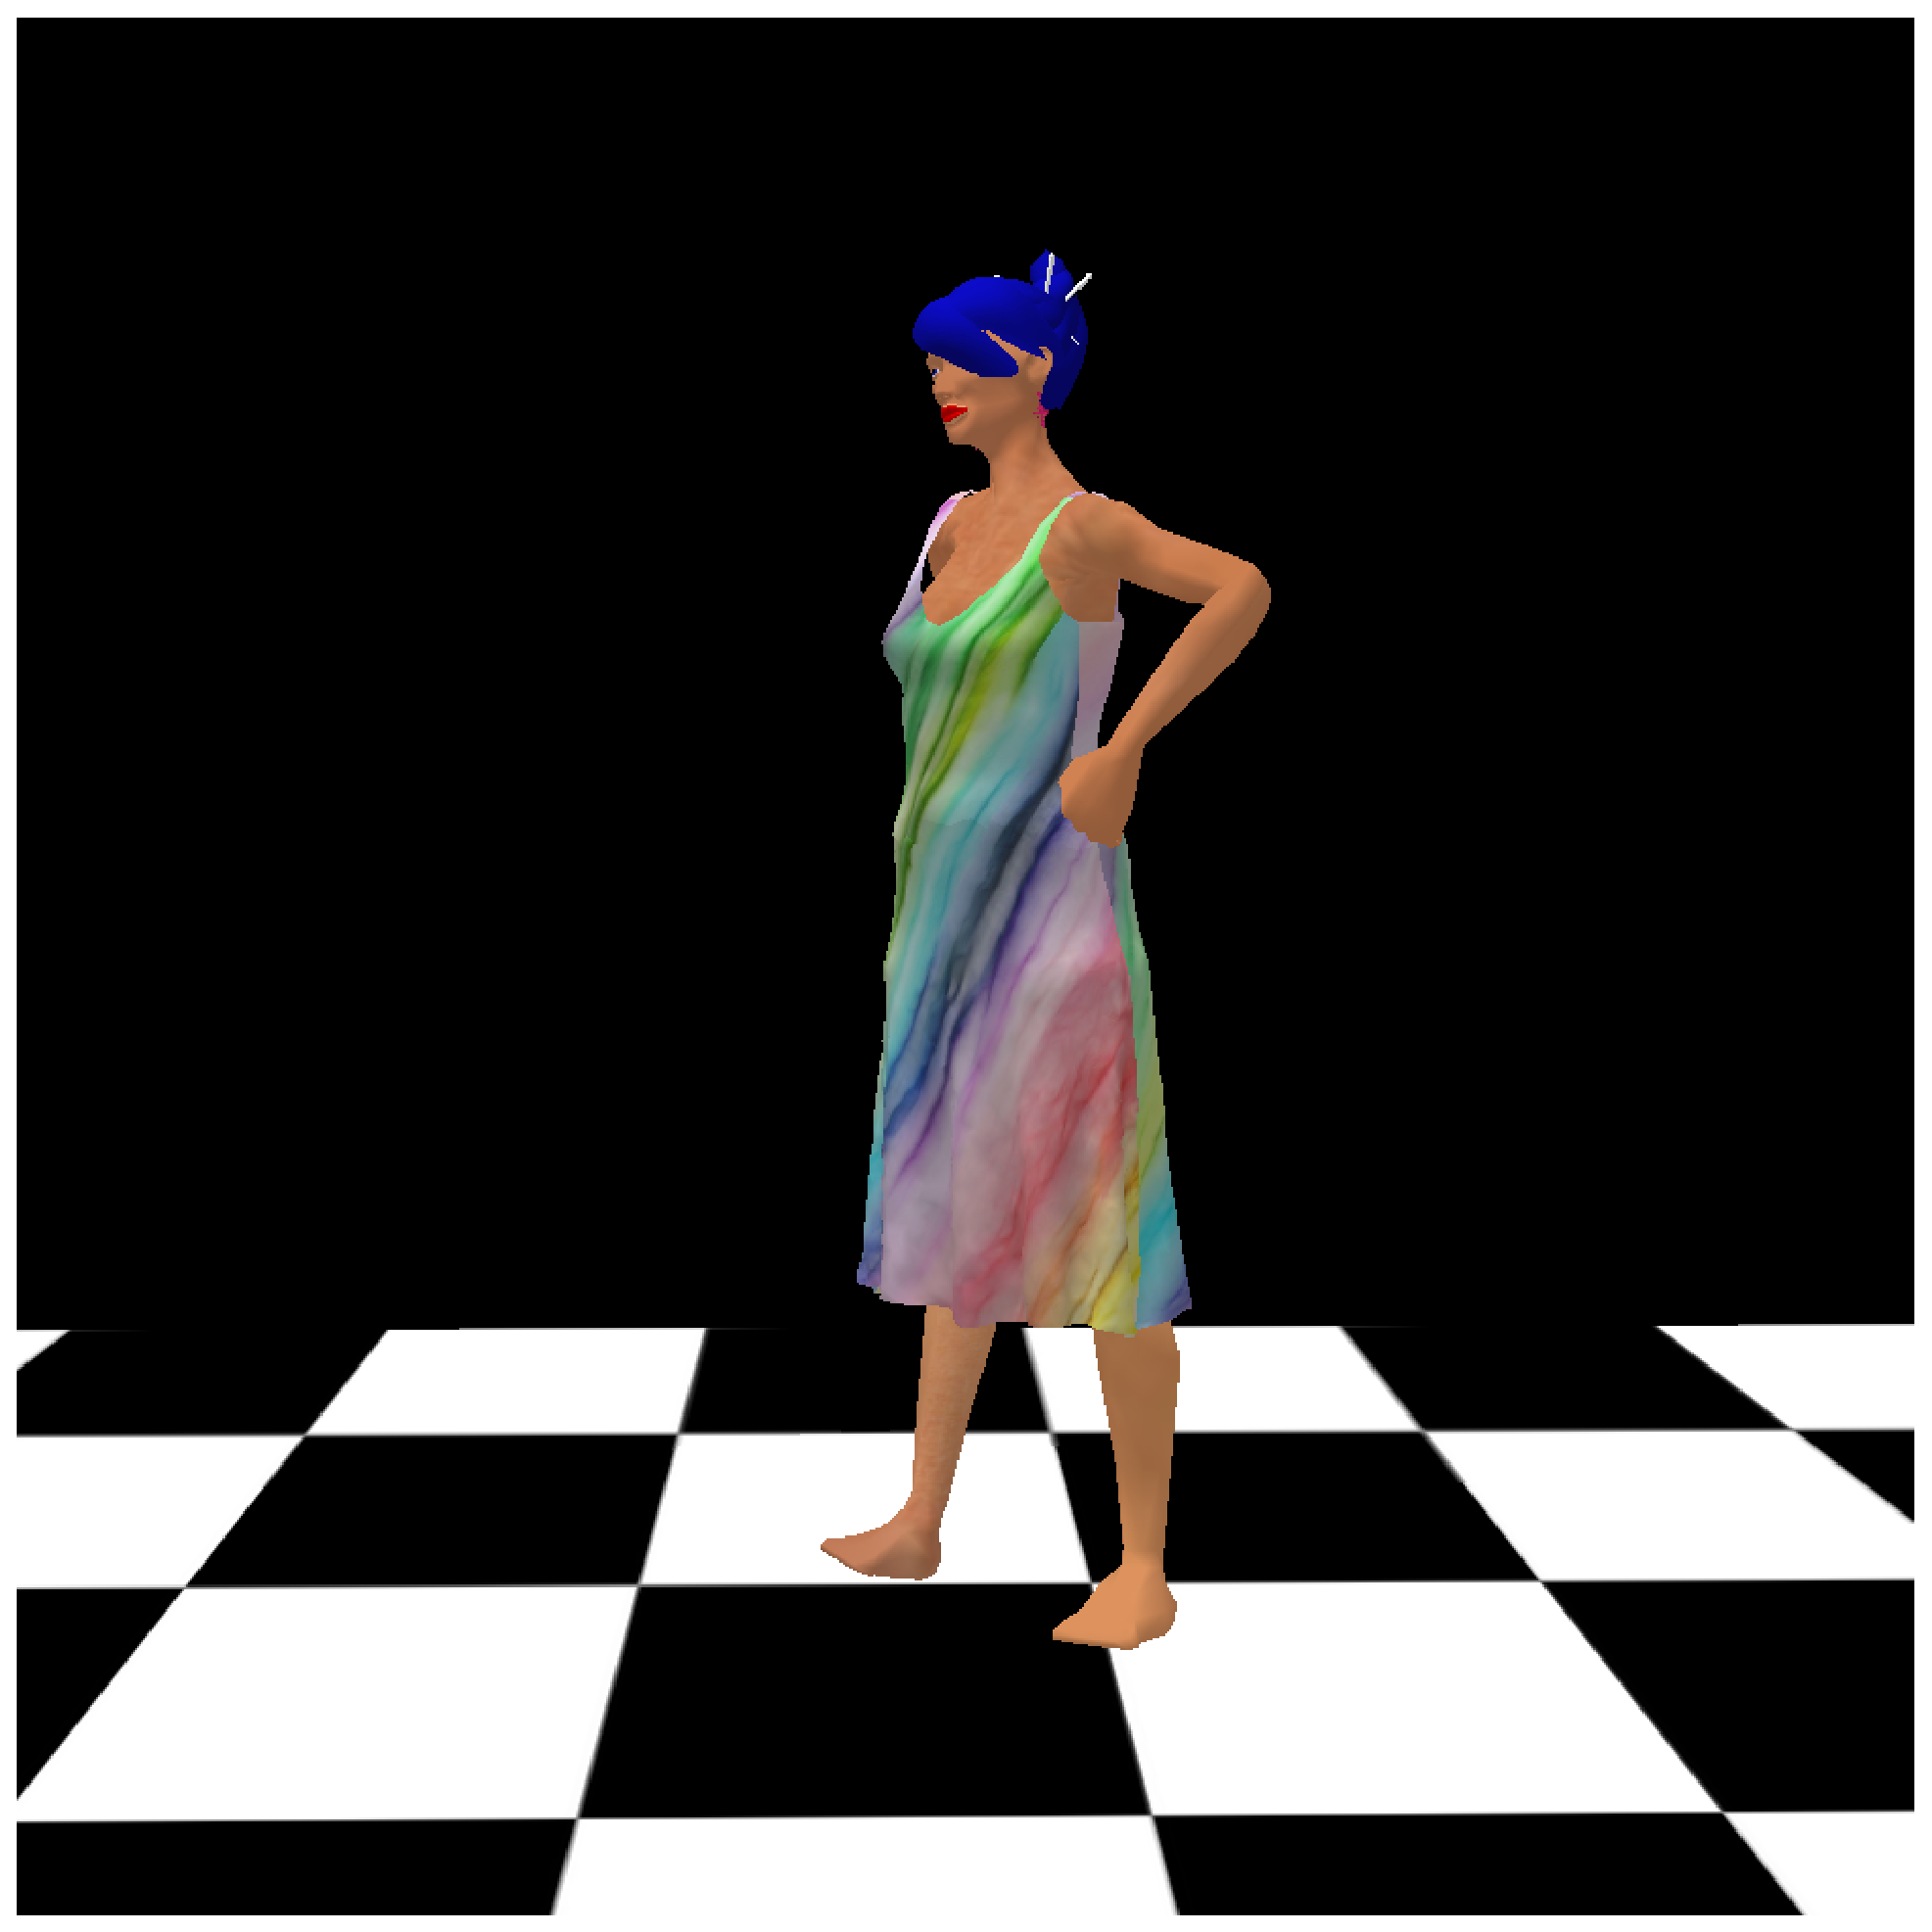
\includegraphics[width=0.50\columnwidth]{./figures/sundress-3.eps}
	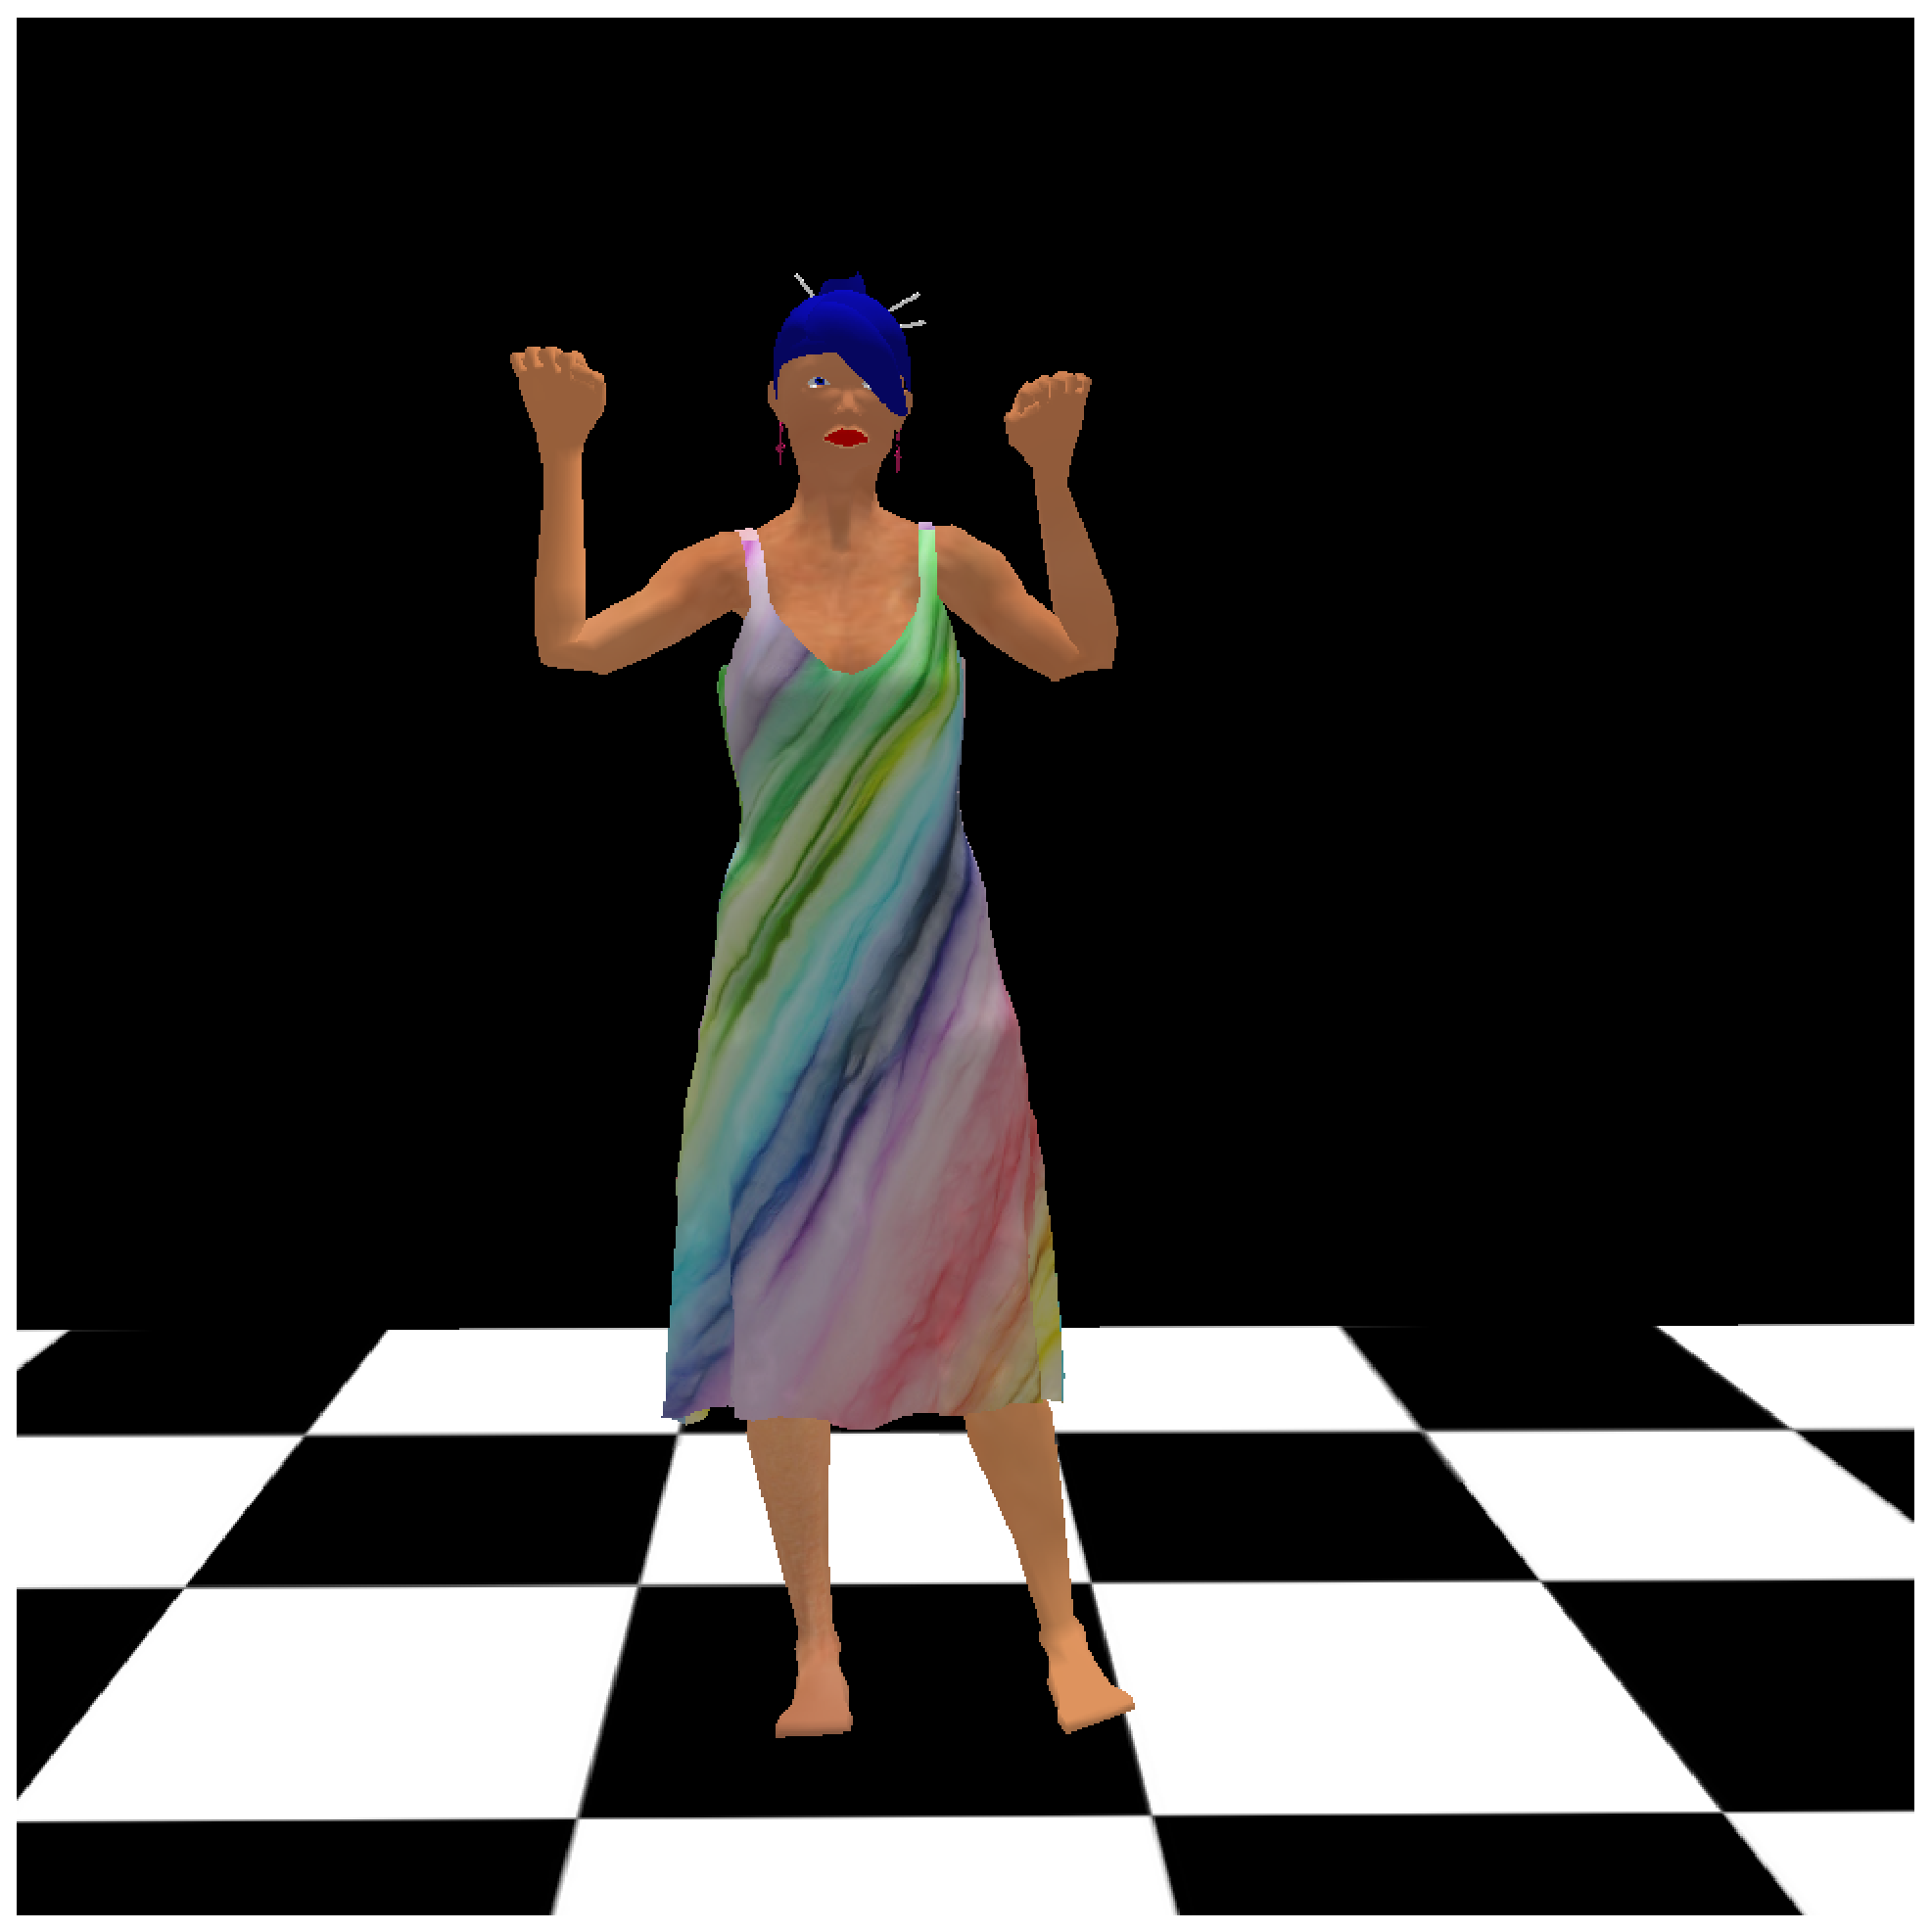
\includegraphics[width=0.50\columnwidth]{./figures/sundress-4.eps}
	}
	\centerline{(a)}
	\centerline{\ }
	\centerline{
	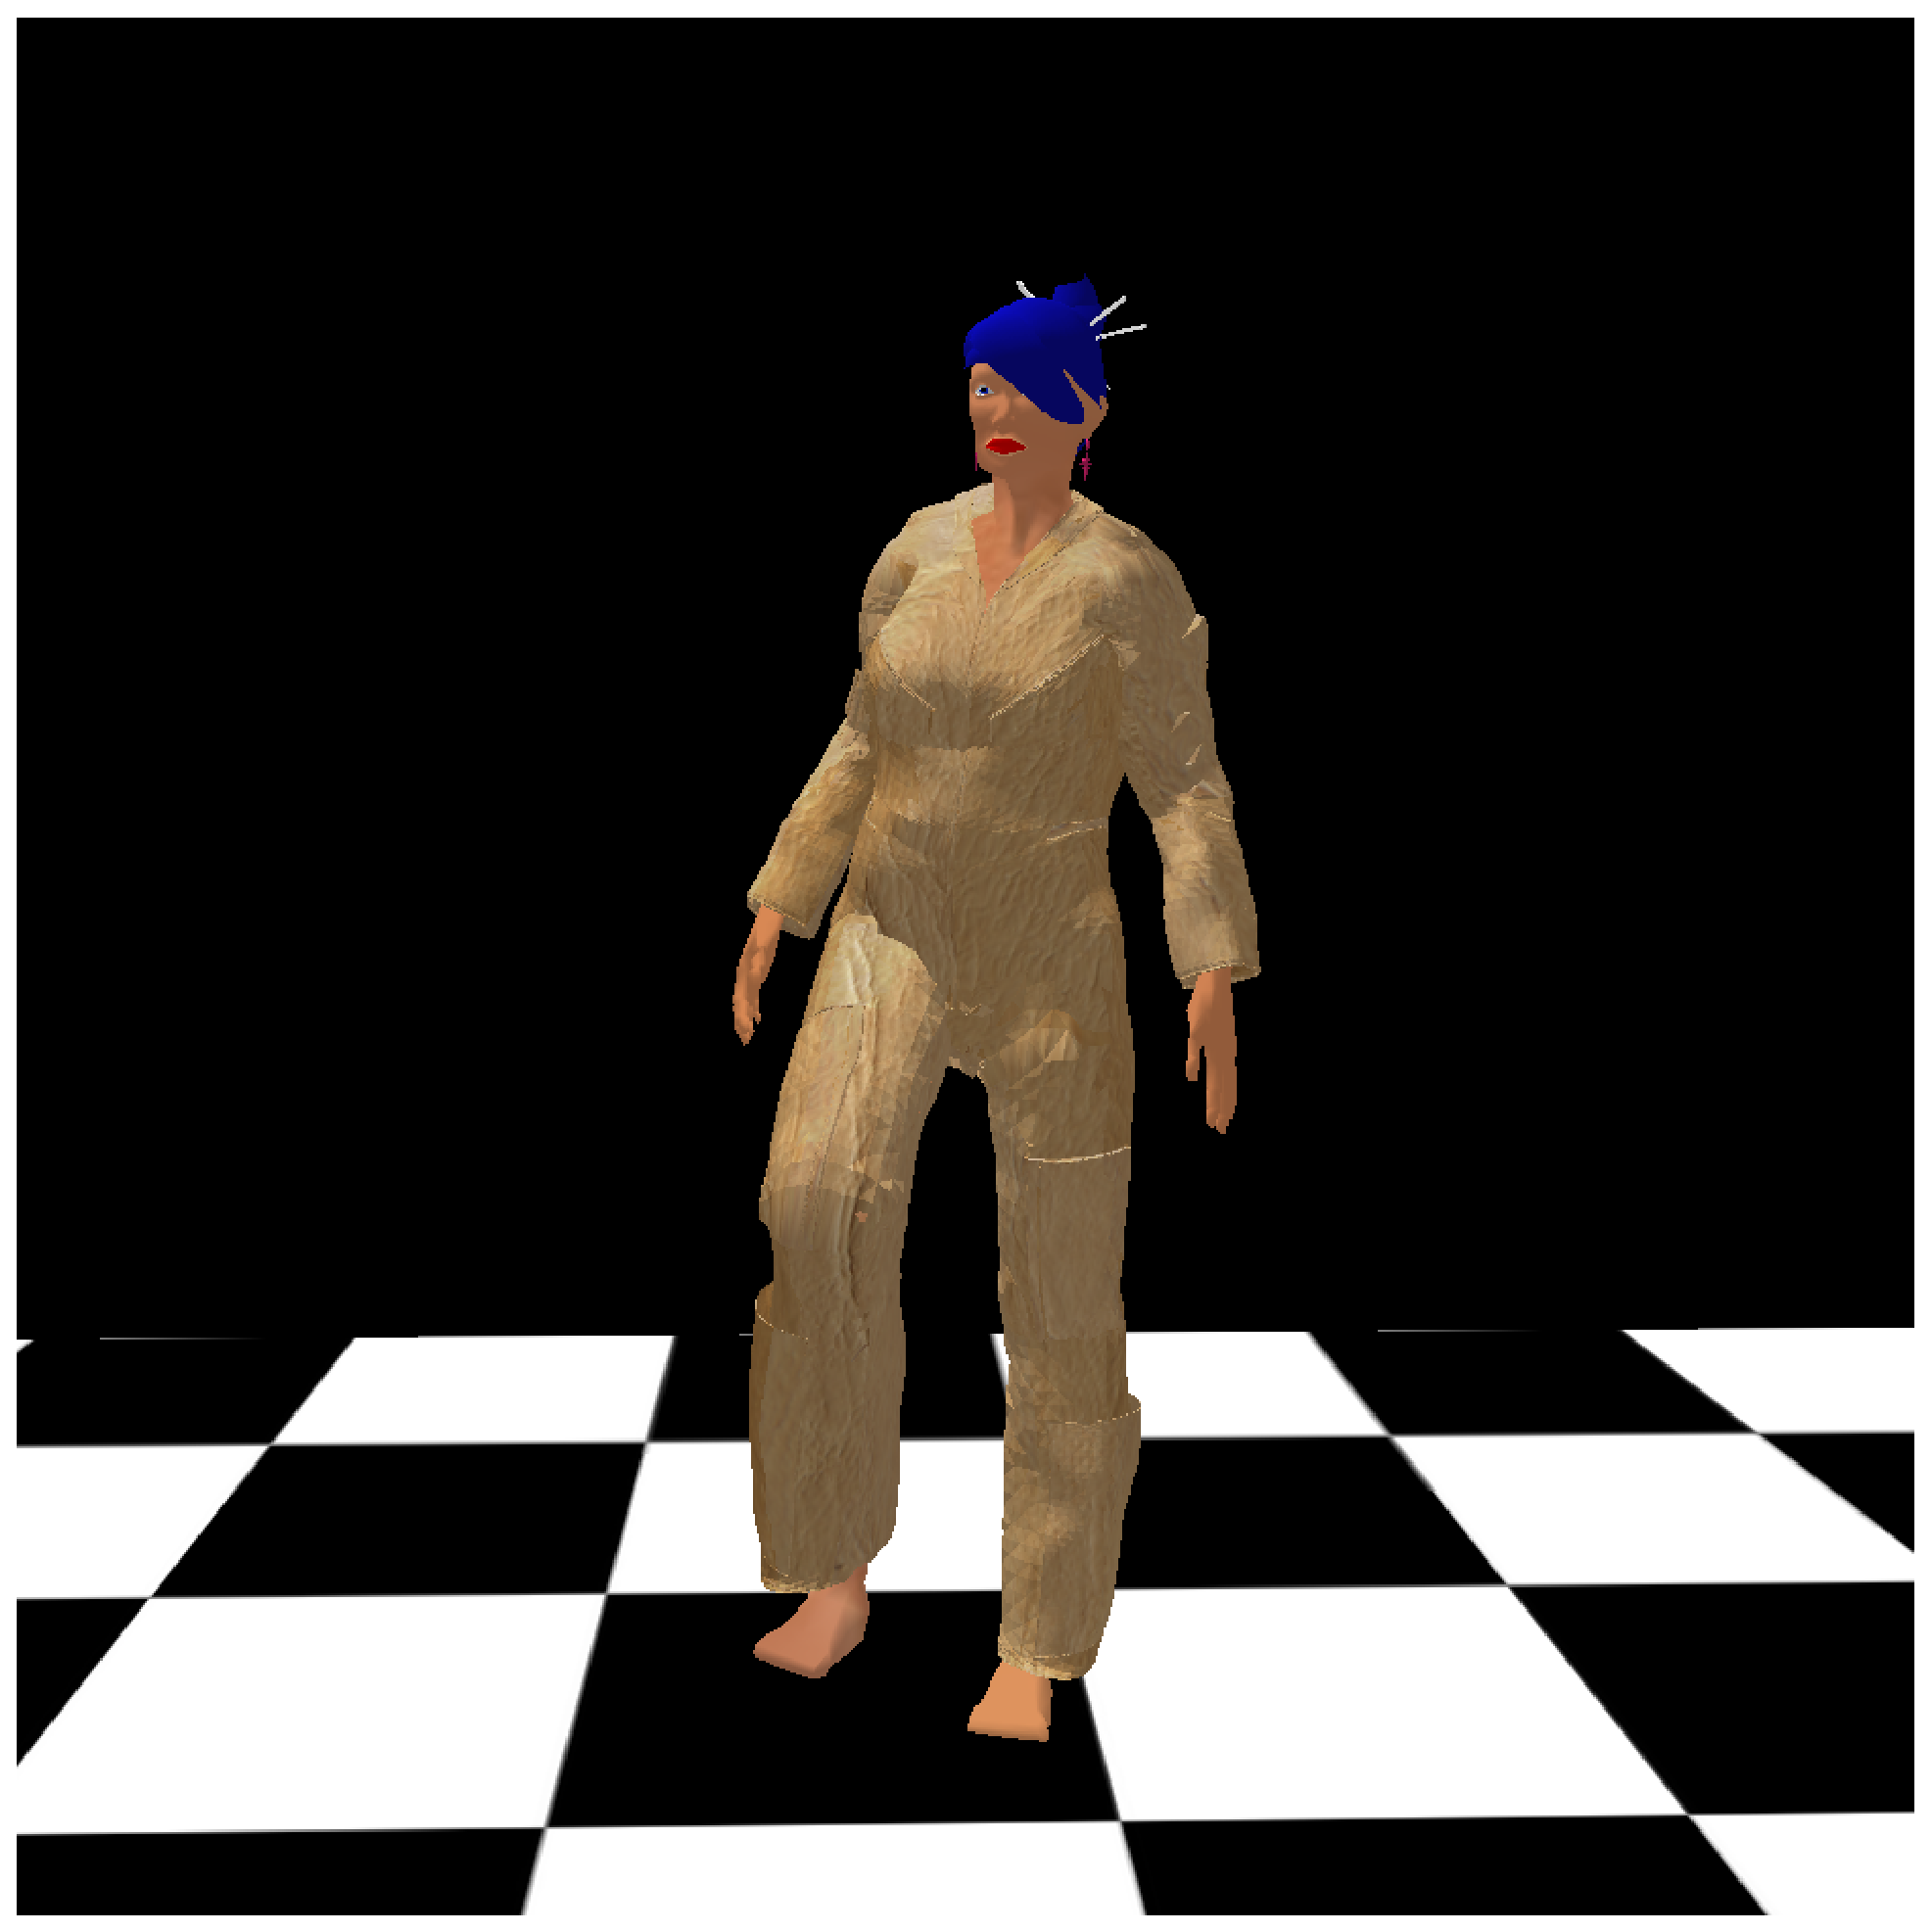
\includegraphics[width=0.50\columnwidth]{./figures/fligh-suit-1.eps}
	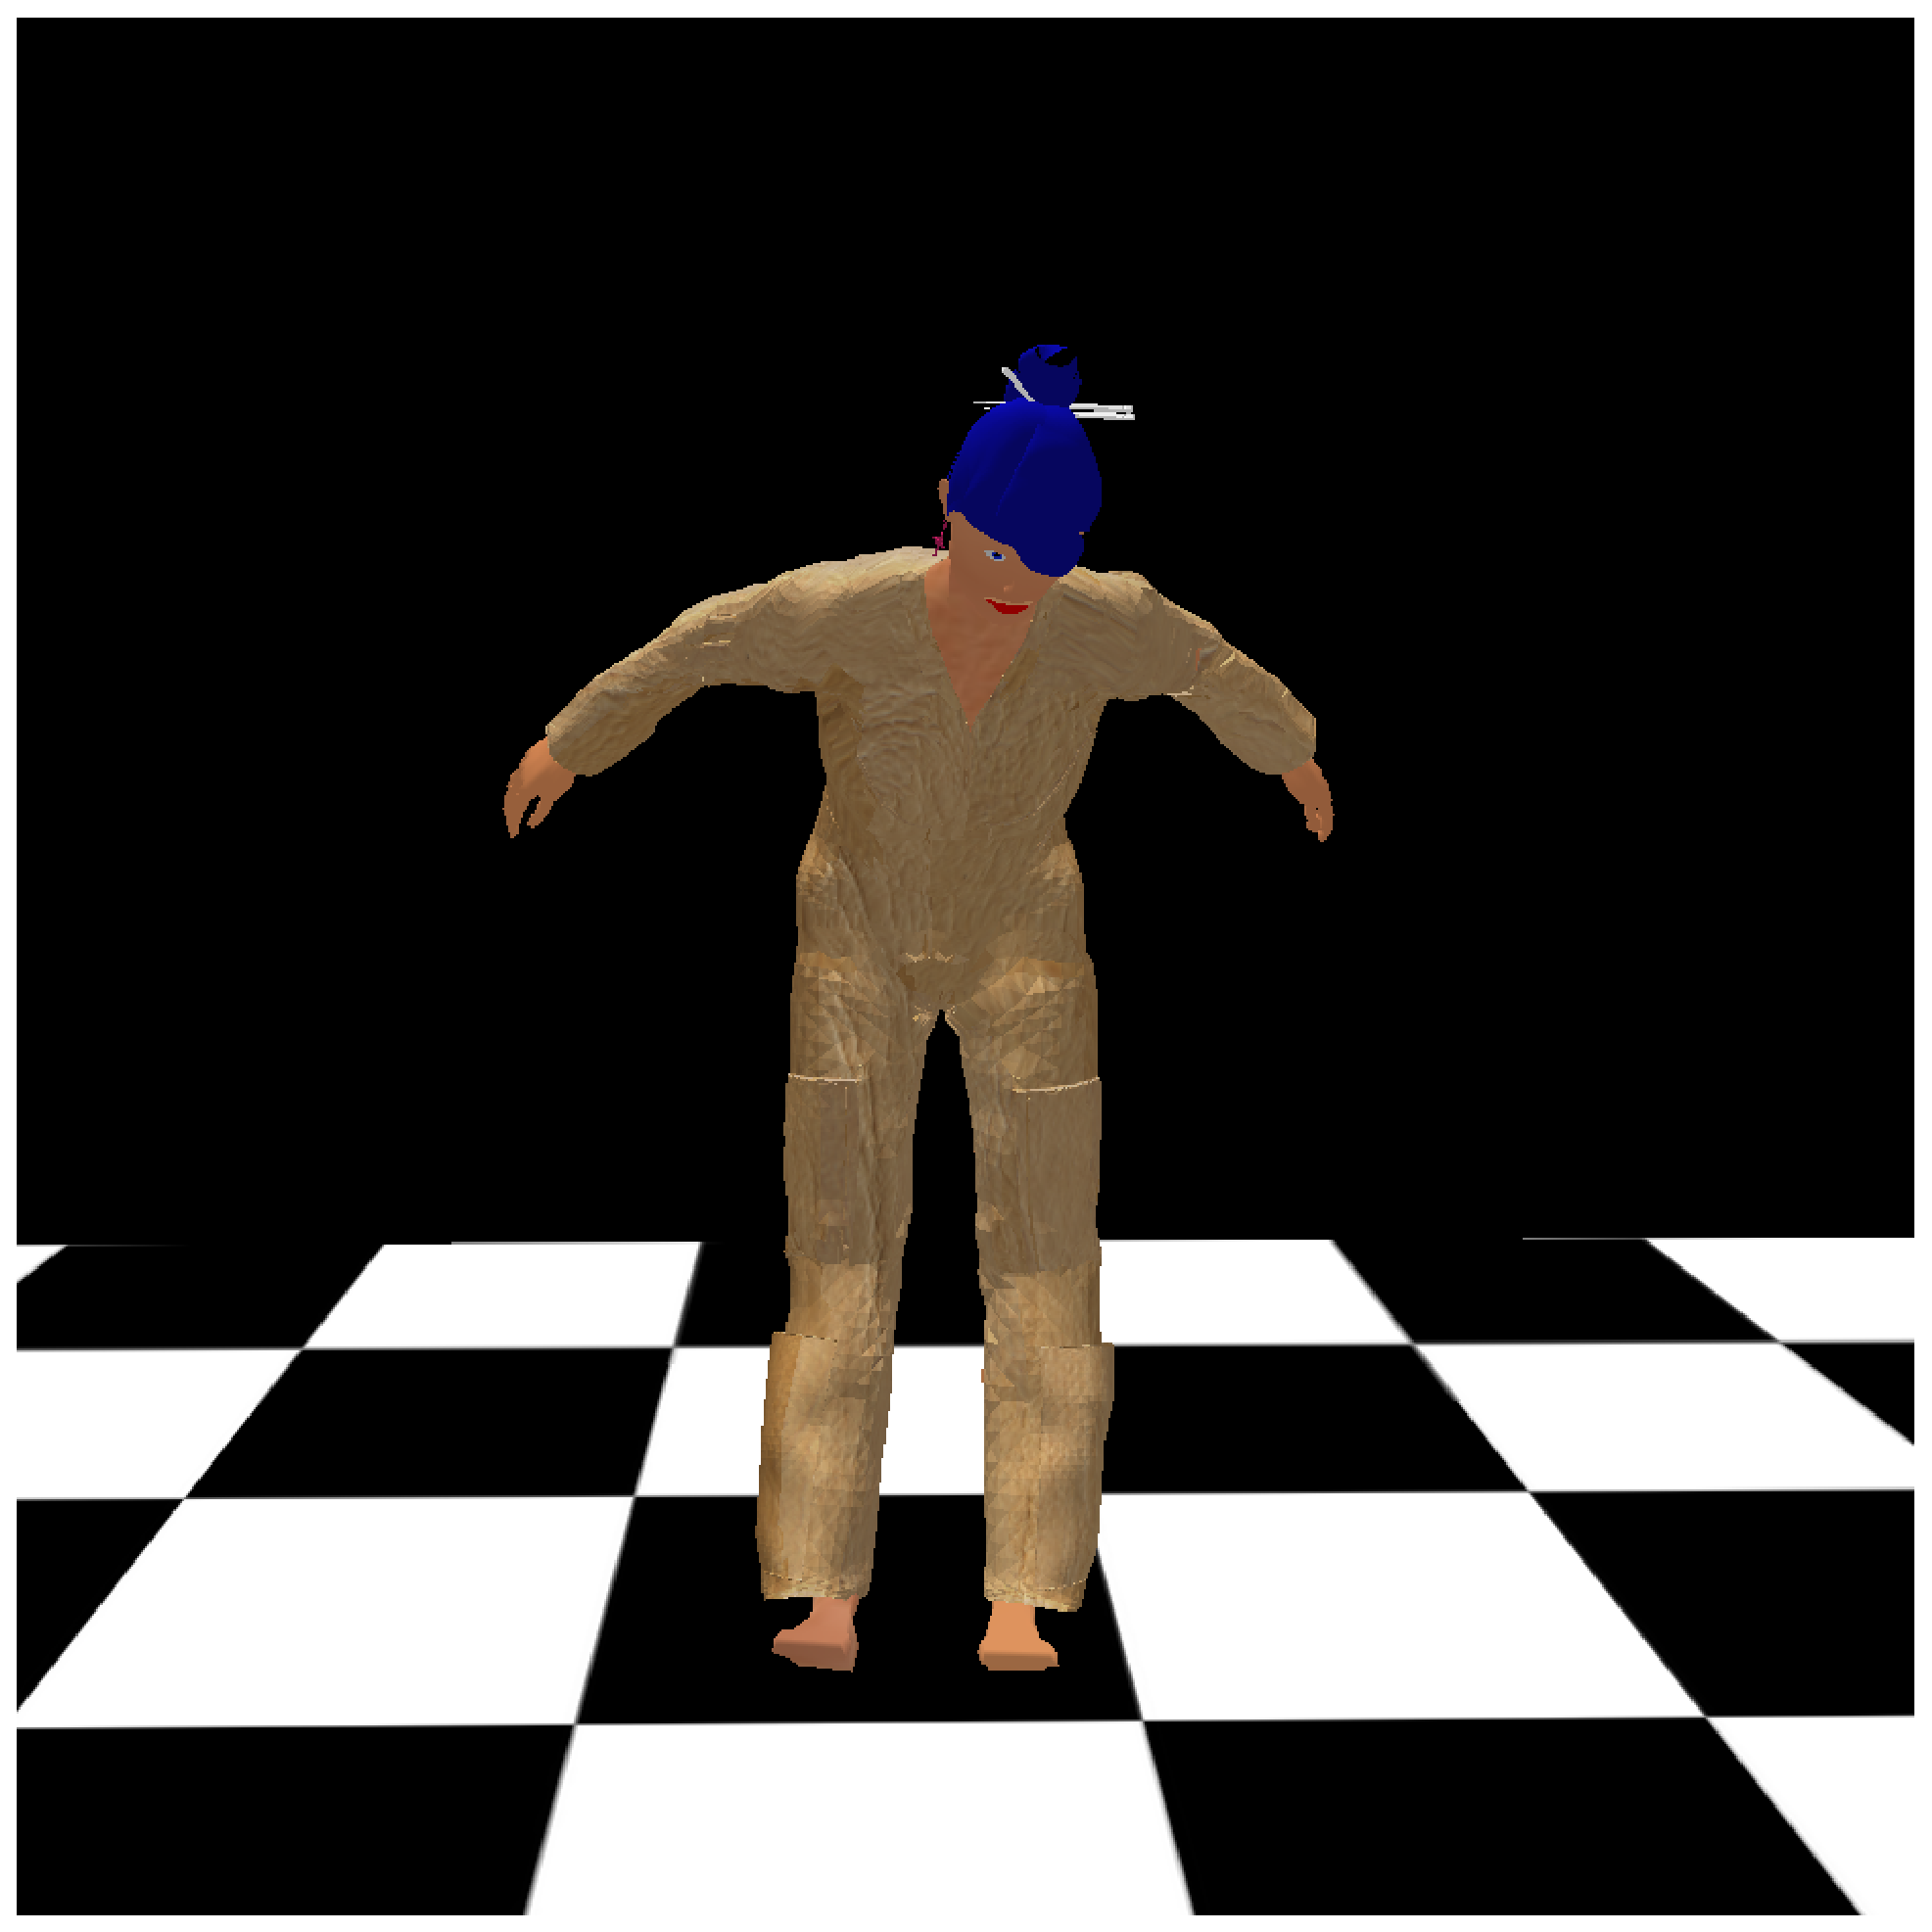
\includegraphics[width=0.50\columnwidth]{./figures/fligh-suit-2.eps}
	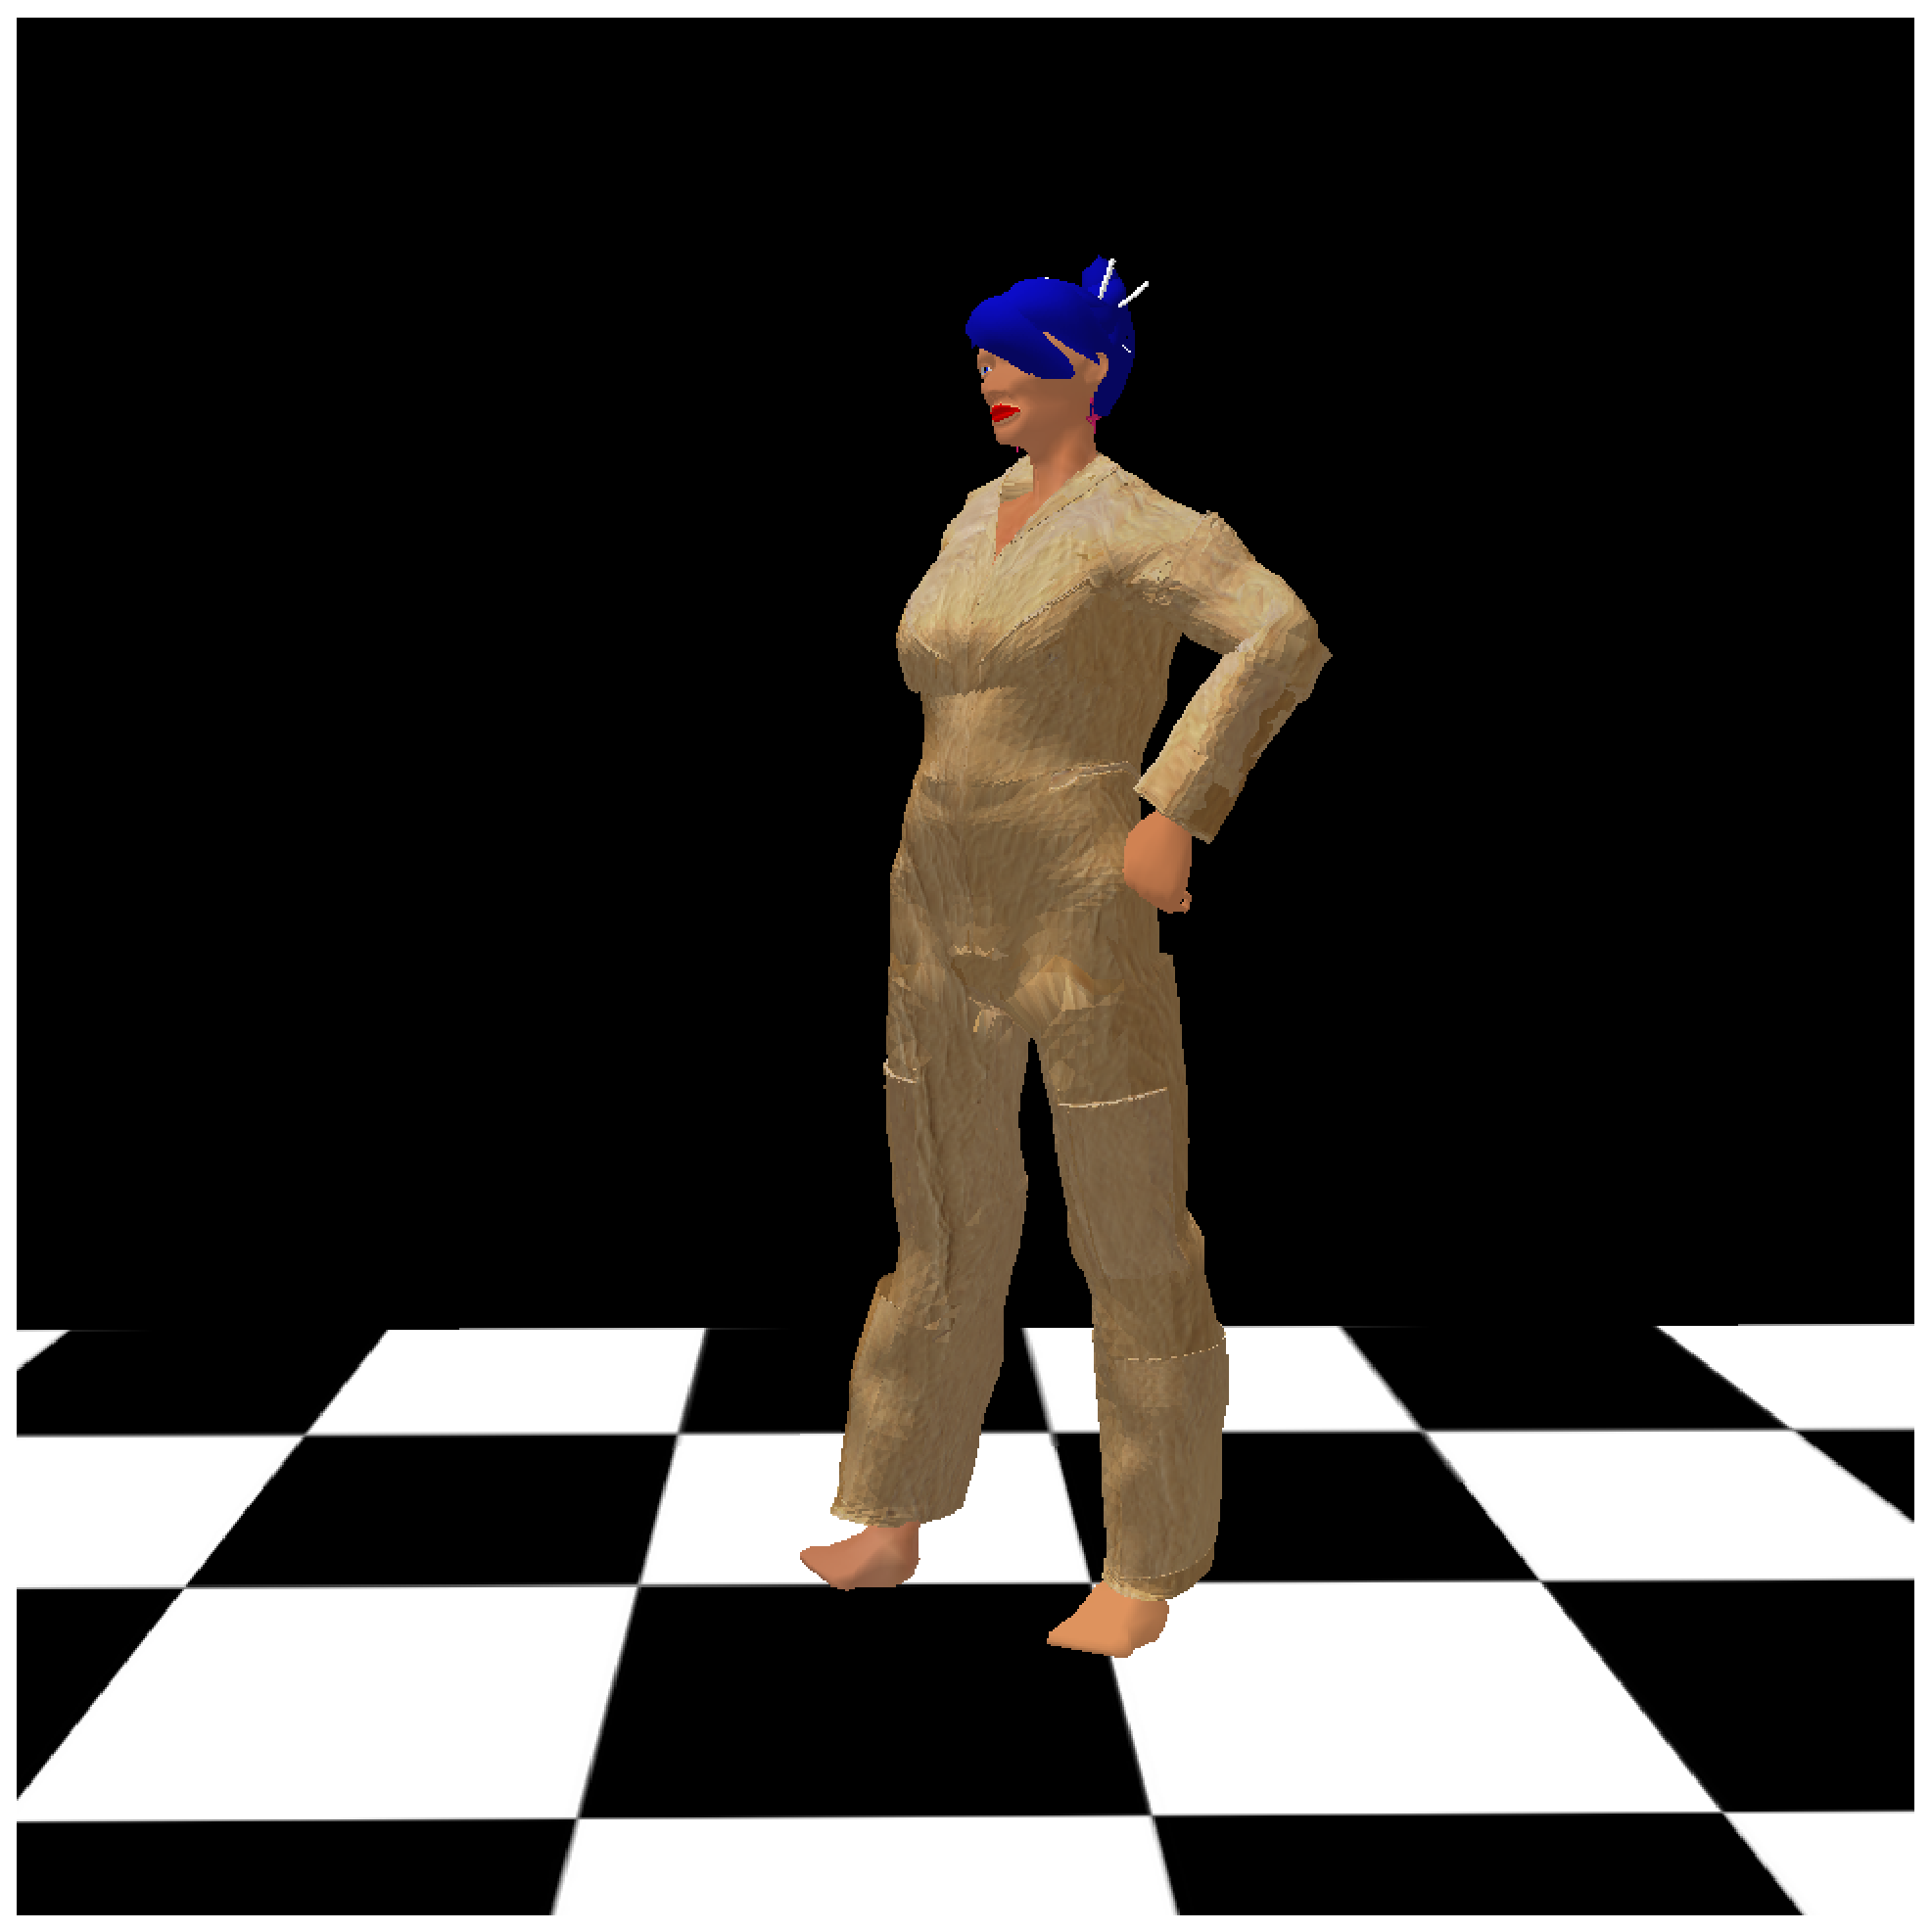
\includegraphics[width=0.50\columnwidth]{./figures/fligh-suit-3.eps}
	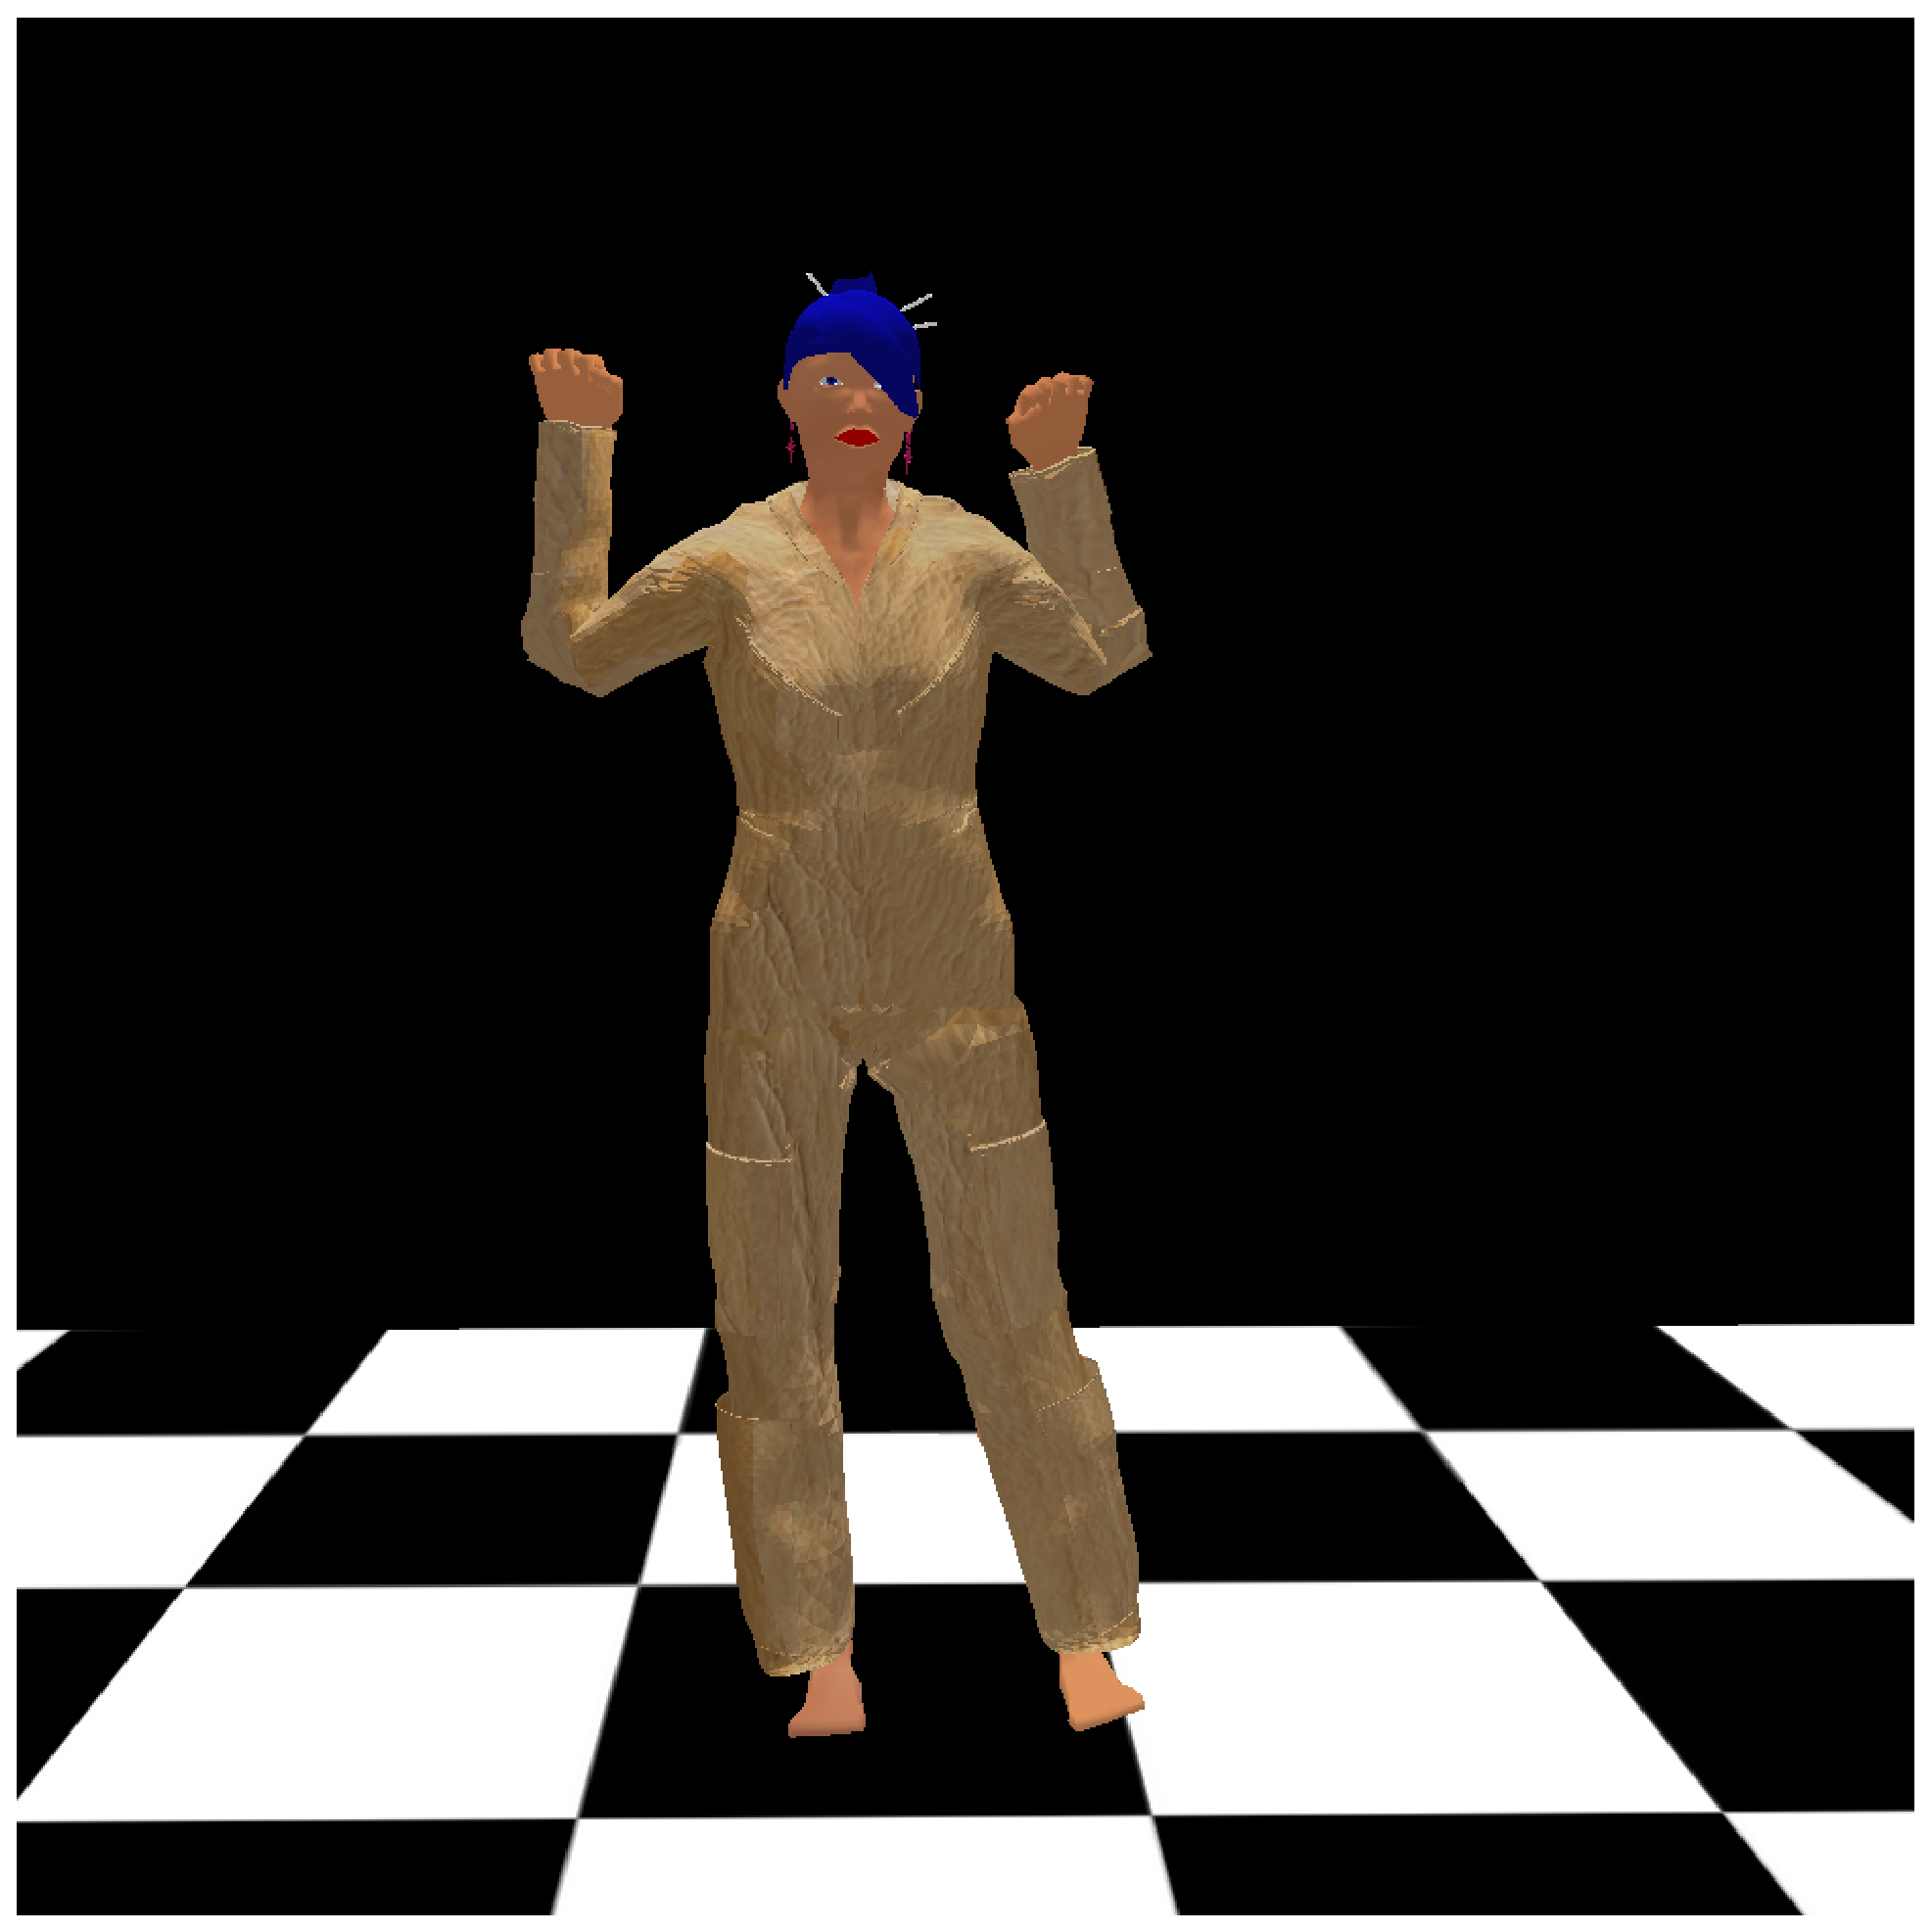
\includegraphics[width=0.50\columnwidth]{./figures/fligh-suit-4.eps}
	}
	\centerline{(b)}
	\caption{Examples of different dresses on a model with different postures: (a) sun dress and (b) flight suit.}
	\label{fig:examples}
\end{figure*}



\section{Conclusion and Future Work}
\label{sec:Conclusions}
The simulation software using optimized parameters with this algorithm is shown in Figure~\ref{fig:system}. Both the optimization and simulation are performed on a high-end PC with Intel i7-2600 and NVIDIA GeForce GTX560Ti. The maximum optimization time is 1.002 seconds, which is constrained by the frame rate of the depth sensor. The actual simulation runs at 600 fps on $1920 \times 1080$ resolution. The body sizes are estimated with error rates less than 4\%, which is sufficient for the realism of the simulation and determining the appropriate apparel size. 

As a future work, we would like to improve the quality of measurements by using data from an RGB sensor as well, as it provides valuable additional data. We would also like to provide more collision sphere data to the framework for better collision detection.
 
\begin{thebibliography}{}
\bibitem{Fitnect2012}
Fitnect Interactive Kft.: 3D Virtual Fitting Dressing Room / Mirror. Available at \verb+http://www.fitnect.hu/+ (2013).

\bibitem{Styku2013}
Styku, Inc.: Virtual Fitting Room and Body Scanning. Available at \verb+http://www.styku.com/+ (2013).

\bibitem{FaceCake2013}
FaceCake Marketing Technologies, Inc., Visual Demonstration System. Available at \verb+http://www.facecake.com/+ (2013).

\bibitem{Protopsaltou2002}
Protopsaltou, D., Luible, C., Arevalo-Poizat, M., Magnenat-Thalmann, N., A Body and Garment Creation Method for an Internet-based Virtual Fitting Room. Proceedings of Computer Graphics International (CGI '02), 105-122, Springer (2002).

\bibitem{Zhang2008}
Zhang, W., Matsumoto, T., Liu, J., Chu, M., and Begole, B.: An Intelligent Fitting Room Using Multi-Camera Perception. Proceedings of the 13th International Conference on Intelligent User Interfaces (IUI '08). ACM, New York, NY, USA, 60-69 (2008).

\bibitem{Giovanni2012}
Giovanni, S., Choi, Y.C., Huang J., Tat K.E. and Yin, K.: Virtual Try-On Using Kinect and HD Camera. MIG, volume 7660 of Lecture Notes in Computer Science, page 55-65. Springer, (2012)

\bibitem{Cheung2005}
Cheung, K.-M., Baker, S., Kanade, T.: Shape-From-Silhouette Across Time, Part II: Applications to Human Modeling and Markerless Motion Tracking, 
International Journal of Computer Vision. 63(2), 225-245 (2005).

\bibitem{Yao2011}
Changa, Y.-J. and Chenb, S.-F., Huang, J.-D.: A Kinect-based System for Physical Rehabilitation: A Pilot Study for Young Adults with Motor Disabilities. Research in Developmental Disabilities, 32(6), 2566-2570 (2011).

\bibitem{Henry2012}
Henry, P., Krainin, M., Herbst, E., Ren, X.F., Fox, D.: RGB-D mapping: Using Kinect-style Depth Cameras for Dense 3D Modeling of Indoor Environments. The International Journal of Robotics Research, 31, 647-663 (2012).

\bibitem{Gallo2012}
Gallo, L., Placitelli, A.P., Ciampi, M.: Controller-free Exploration of Medical Image Data: Experiencing the Kinect. 
Proceedings of the 24th International Symposium on Computer-Based Medical Systems (CBMS), 1-6 (2011).

\bibitem{Meng2010}
Meng, Y., Mok, P.Y., Jin, X.: Interactive Virtual Try-on Clothing Design Systems. Computer-Aided Design, 42(4), 310�321 (2010).

\bibitem{OpenNI2013}
OpenNI Consortium: OpenNI - The Standard Framework for 3D Sensing. Available at \verb+http://www.openni.org/+ (2013).

\bibitem{Microsoft2013}
Microsoft, Inc.: Kinect for Windows. Available at \verb+http://www.microsoft.com/en-us/kinectforwindows/+ (2013).

\bibitem{Khoshelham2012}
Khoshelham, K., Elberink, S.O.: Accuracy and Resolution of Kinect Depth Data for Indoor Mapping Applications. Sensors, 12, 1437-1454 (2012).

\bibitem{Matyunin2011}
Matyunin, S., Vatolin, D., Berdnikov, Y., Smirnov, M.: Temporal Filtering for Depth Maps Generated by Kinect Depth Camera. Proceedings of the 3DTV Conference: The True Vision - Capture, Transmission and Display of 3D Video (3DTV-CON), 1-4 (2011).

\bibitem{PS2102}
PrimeSense, Inc.: NITE Middleware - the Natural Interaction Engine. Available at \verb+http://www.primesense.com/solutions/nite-middleware/+ (2013).

\bibitem{Willis2012}
Willis, B.: Body Proportions in Art. Wunderland Web Design (2013).

\bibitem{Cui2013}
Cui Y., Chang W., N\"{o}ll T., Stricker D., KinectAvatar: Fully Automatic Body Capture Using a Single Kinect, 
Computer Vision - ACCV 2012 Workshops, Lecture Notes in Computer Science, 7729, 133-147, Daejeon, S. Korea (2013)

\bibitem{Cui2010}
Cui, Y., Schuon, S., Chan, D., Thrun, S., Theobalt, C.: 3D shape scanning with a time-of-flight camera. Proceedings of IEEE Conference on Computer Vision and Pattern Recognition (CVPR), 1173-1180 (2010) 

\bibitem{Kim2011}
Kim T.-Y.: Character clothing in PhysX 3, ACM SIGGRAPH ASIA NVIDIA Tech Talks, Hong Kong (2011)

\bibitem{M�llera2007}
M�llera M., Heidelbergera B, Hennixa M., Ratcliff J.: Position Based Dynamics. Journal of Visual Communication and Image Representation, 18(2), 109�118 (2007)

\bibitem{Tonge2010}
Tonge, R.: Nvidia. Collision detection in PhysX, Recent Advances in Real-Time Collision and Proximity Computations for
Games and Simulations, ACM SIGGRAPH Course Notes (2010)

\bibitem{Azimi2012}
Azimi M.: Skeletal Joint Smoothing, White Paper, Available at \verb+http://msdn.microsoft.com/en-us/library/jj131429.aspx+ [Online] (2012)

\bibitem{Kalekar2004}
Kalekar, Prajakta S.: Time series forecasting using Holt-Winters exponential smoothing. Kanwal Rekhi School of Information Technology (2004).

\bibitem{Kavan2009}
Kavan, L., Collins, S., O'Sullivan ,C.: Automatic linearization of nonlinear skinning.  Proceedings of the Symposium on Interactive 3D Graphics and Games (I3D '09). ACM, New York, NY, USA, 49-56 (2009)

\bibitem {HANIM}
H-Anim: Humanoid Animation Working Group. Available at \verb+http://www.h-anim.org+ (2013).

\bibitem {Yasseen2013}
Z. Yasseen, A. Nasri, W. Boukaram, P. Volino, N. Magnenat-Thalmann, Sketch-based garment design with quad meshes, Computer-Aided Design, Volume 45, Issue 2, February 2013, Pages 562-567,

\bibitem{Kim2013}
Kim, Dong-Eun, and Karen LaBat. "Consumer experience in using 3D virtual garment simulation technology." Journal of The Textile Institute ahead-of-print (2013): 1-11.

\bibitem{Meng2010}
Meng, Yuwei, P. Y. Mok, and Xiaogang Jin. "Interactive virtual try-on clothing design systems." Computer-Aided Design 42.4 (2010): 310-321.

\bibitem{Zhou2012}
Zhenglong Zhou, Bo Shu, Shaojie Zhuo, Xiaoming Deng, Ping Tan, and Stephen Lin. 2012. Image-based clothes animation for virtual fitting. In SIGGRAPH Asia 2012 Technical Briefs (SA '12). ACM, New York, NY, USA, , Article 33 , 4 pages.

\bibitem{Hauswiesner2013}
Hauswiesner, Stefan, Matthias Straka, and Gerhard Reitmayr. "Virtual Try-On Through Image-based Rendering." (2013): 1-1.

\bibitem{Samejima2012}
Samejima, Ippei, et al. "A body dimensions estimation method of subject from a few measurement items using KINECT." Systems, Man, and Cybernetics (SMC), 2012 IEEE International Conference on. IEEE, 2012.

\end{thebibliography}

\end{document}



